\documentclass[10pt,letterpaper,cm]{nupset}
\usepackage[margin=1in]{geometry}
\usepackage{graphicx}
\usepackage{float}
\usepackage{svg}
 \usepackage{enumerate}
 \usepackage{enumitem}
 \usepackage{stmaryrd}
\usepackage{amsfonts}
\usepackage{amssymb}
\usepackage{pgfplots}
\pgfplotsset{compat=1.13}
\usepackage{amsmath,amsthm}
\usepackage{lmodern}
\usepackage{tikz-cd}
\usetikzlibrary{automata,positioning}
\usetikzlibrary{quotes}
\usepackage{faktor}
\usepackage{xfrac}
\usepackage{mathtools}
\usepackage{bm}
\usepackage{xcolor}
\usepackage{soul}
\usepackage{ dsfont }
\usepackage{stackengine}
\usepackage{mathrsfs}
\usepackage{hyperref}
\usepackage{url}
\usepackage{thmtools}
\usepackage[capitalise]{cleveref}
\usepackage[linesnumbered,ruled]{algorithm2e}
\hypersetup{colorlinks=true, linkcolor=red,          % color of internal links (change box color with linkbordercolor)
    citecolor=green,        % color of links to bibliography
    filecolor=magenta,      % color of file links
    urlcolor=cyan           }
    
\usepackage{thmtools}
\usepackage[capitalise]{cleveref} 
\usepackage{comment}
    
\theoremstyle{definition}
\newtheorem{definition}{Definition}[subsection]
\newtheorem{exmp}[definition]{Example}
\newtheorem{non-exmp}[definition]{Non-example}
\newtheorem{note}[definition]{Note}

\theoremstyle{theorem}
\newtheorem{theorem}[definition]{Theorem}
\newtheorem{lemma}[definition]{Lemma}
\newtheorem{prop}[definition]{Proposition}
\newtheorem{corollary}[definition]{Corollary}
\newtheorem*{claim}{Claim}
\newtheorem{exercise}[definition]{Exercise}

\theoremstyle{remark}
\newtheorem{remark}[definition]{Remark}
\newtheorem*{todo}{To do}
\newtheorem*{conv}{Convention}
\newtheorem*{aside}{Aside}
\newtheorem*{notation}{Notation}
\newtheorem*{term}{Terminology}
\newtheorem*{background}{Background}
\newtheorem*{further}{Further reading}
\newtheorem*{sources}{Sources}

\makeatletter
\def\th@plain{%
  \thm@notefont{}% same as heading font
  \itshape % body font
}
\def\th@definition{%
  \thm@notefont{}% same as heading font
  \normalfont % body font
}
\makeatother

\setlength{\parindent}{0pt}

\makeatletter
\renewcommand*\env@matrix[1][*\c@MaxMatrixCols c]{%
  \hskip -\arraycolsep
  \let\@ifnextchar\new@ifnextchar
  \array{#1}}
\makeatother
\pgfplotsset{unit circle/.style={width=4cm,height=4cm,axis lines=middle,xtick=\empty,ytick=\empty,axis equal,enlargelimits,xmax=1,ymax=1,xmin=-1,ymin=-1,domain=0:pi/2}}

\def\ruleoffset{1pt}
\newcommand\specialvdash[2]{\mathrel{\ensurestackMath{
  \mkern2mu\rule[-\dp\strutbox]{.4pt}{\baselineskip}\stackon[\ruleoffset]{
    \stackunder[\dimexpr\ruleoffset-.4\ht\strutbox+.4\dp\strutbox]{
      \rule[\dimexpr.4\ht\strutbox-.4\dp\strutbox]{2.5ex}{.4pt}}{
        \scriptstyle #1}}{\scriptstyle#2}\mkern2mu}}
}

\newcommand{\A}{\mathfrak A}
\newcommand{\C}{\mathfrak C}
\newcommand{\E}{\vec E}
\newcommand{\CP}{\mathbb CP}
\newcommand{\F}{\mathbb F}
\newcommand{\G}{\mathbb G}
\renewcommand{\H}{\mathcal H}
\newcommand{\HP}{\mathbb HP}
\newcommand{\K}{\mathbb K}
\renewcommand{\L}{\mathcal L}
\newcommand{\M}{\mathbb M}
\newcommand{\N}{\mathbb N}
\newcommand{\U}{\mathcal U}
\renewcommand{\O}{\mathbf O}
\newcommand{\OP}{\mathbb OP}
\renewcommand{\P}{\mathbb P}
\newcommand{\Q}{\mathbb Q}
\newcommand{\I}{\mathbb I}
\newcommand{\R}{\mathbb R}
\newcommand{\RP}{\mathbb RP}
\renewcommand{\S}{\mathbf S}
\newcommand{\T}{\mathbf T}
\newcommand{\Z}{\mathbb Z}
\newcommand{\B}{\mathfrak{B}}
\newcommand{\1}{\mathbf{1}}
\newcommand{\ds}{\displaystyle}
\newcommand{\ran}{\right>}
\newcommand{\lan}{\left<}
\newcommand{\bmat}[1]{\begin{bmatrix} #1 \end{bmatrix}}

\renewcommand{\a}{\mathscr{A}}
\renewcommand{\b}{\mathscr{B}}
\renewcommand{\c}{\mathfrak{c}}
\renewcommand{\d}{\mathscr{D}}
\newcommand{\e}{\mathscr{E}}
\newcommand{\y}{\mathscr{Y}}
\renewcommand{\j}{\mathscr{J}}
\newcommand{\X}{\mathscr X}

\newcommand{\h}{\vec h}
\newcommand{\f}{\vec f}
\newcommand{\g}{\vec g}
\renewcommand{\i}{\vec i}
\renewcommand{\k}{\vec k}
\newcommand{\n}{\vec n}
\newcommand{\p}{\vec p}
\newcommand{\q}{\vec q}
\renewcommand{\r}{\vec r}
\newcommand{\s}{\vec s}
\renewcommand{\t}{\vec t}
\renewcommand{\u}{\vec u}
\renewcommand{\v}{\vec v}
\newcommand{\w}{\vec w}
\newcommand{\x}{\vec x}
\newcommand{\0}{\vec 0}

\newcommand{\z}{\mathsf{Z}}
\newcommand{\zf}{\mathsf{ZF}}
\newcommand{\zfc}{\mathsf{ZFC}}
\newcommand{\ac}{\mathsf{AC}}
\newcommand{\ord}{\mathsf{OR}}
\newcommand{\VL}{\mathsf{V=L}}

\makeatletter
\newcommand*\bigcdot{\mathpalette\bigcdot@{.5}}
\newcommand*\bigcdot@[2]{\mathbin{\vcenter{\hbox{\scalebox{#2}{$\m@th#1\bullet$}}}}}
\makeatother

\DeclareMathOperator{\Ima}{Im}
\DeclareMathOperator*{\Span}{span}
\DeclareMathOperator*{\GL}{GL}
\DeclareMathOperator*{\SL}{SL}
\DeclareMathOperator{\rng}{range}
\DeclareMathOperator{\gemu}{gemu}
\DeclareMathOperator{\almu}{almu}
\newcommand{\Char}{\mathsf{char}}
\DeclareMathOperator{\id}{id}
\DeclareMathOperator{\abs}{Abs}
\DeclareMathOperator{\graph}{Graph}
\DeclareMathOperator{\gal}{Gal}
\DeclareMathOperator{\tr}{Tr}
\DeclareMathOperator{\out}{out}
\DeclareMathOperator{\norm}{N}
\DeclareMathOperator{\aut}{Aut}
\DeclareMathOperator{\Int}{Int}
\DeclareMathOperator{\Ext}{Ext}
\DeclareMathOperator{\ext}{ext}
\DeclareMathOperator{\stab}{Stab}
\DeclareMathOperator{\orb}{Orb}
\DeclareMathOperator{\inn}{Inn}
\DeclareMathOperator{\op}{op}
\DeclareMathOperator{\fix}{Fix}
\DeclareMathOperator{\ab}{ab}
\DeclareMathOperator{\sgn}{sgn}
\DeclareMathOperator{\syl}{syl}
\DeclareMathOperator{\Syl}{Syl}
\DeclareMathOperator{\conj}{conj}
\DeclareMathOperator{\im}{im}
\DeclareMathOperator{\dom}{dom}
\DeclareMathOperator{\ed}{End}
\DeclareMathOperator{\gr}{\mathsf{gr}}
\DeclareMathOperator{\map}{Map}
\DeclareMathOperator{\mor}{mor}
\DeclareMathOperator{\ob}{ob}
\DeclareMathOperator{\pr}{pr}
\DeclareMathOperator{\fs}{fs}
\DeclareMathOperator{\order}{order}
\DeclareMathOperator{\Sing}{Sing}
\DeclareMathOperator{\Mat}{Mat}
\DeclareMathOperator{\Hom}{Hom}
\DeclareMathOperator{\Fun}{Fun}
\DeclareMathOperator{\Fr}{Fr}
\DeclareMathOperator{\cl}{cl}
\DeclareMathOperator{\cf}{cf}
\DeclareMathOperator{\wi}{WI}
\DeclareMathOperator{\si}{\mathsf{SI}}
\DeclareMathOperator{\rnk}{rank}
\DeclareMathOperator{\con}{Con}
\DeclareMathOperator{\card}{\mathtt{card}}
\DeclareMathOperator{\od}{\mathtt{ord}}
\DeclareMathOperator{\cb}{cb}
\DeclareMathOperator{\ctm}{ctm}
\DeclareMathOperator{\hc}{HC}
\DeclareMathOperator{\tc}{TC}
\DeclareMathOperator{\poly}{poly}
\DeclareMathOperator{\Def}{Def}
\DeclareMathOperator{\supp}{supp}

\newcommand{\bi}{\begin{itemize}}
\newcommand{\ei}{\end{itemize}}

\newcommand{\be}{\begin{enumerate}}
\newcommand{\ee}{\end{enumerate}}

\newcommand{\Abs}[3]{\ensuremath{Abs(#1, #2, #3)}}

\newcounter{casenum}
\newenvironment{caseof}{\setcounter{casenum}{1}}{\vskip.5\baselineskip}
\newcommand{\case}[2]{\vskip.5\baselineskip\par\noindent {\bfseries Case \arabic{casenum}:} #1\\#2\addtocounter{casenum}{1}}

\pagestyle{headings}

\linespread{1.3}

% info for header block in upper right hand corner
\name{Perry Hart}
\class{MATH 571}
\assignment{Spring 2018}

\begin{document}
\thispagestyle{empty}
\begin{abstract}
These notes, which are unfinished, are based on Scott Weinstein's ``Topics in Logic: Set Theory'' lectures at UPenn along with  Thomas Jech's \textit{Set Theory - The Third Millennium Edition, revised and expanded}. Any mistake in what follows is my own.
\end{abstract}

\tableofcontents
\newpage

\section{Point-set topology of $\R$}

\subsection{Lecture 1}

Throughout this section, we shall  work tacitly in $\zfc$.

\begin{notation}
$\N \coloneqq \left\{0,1,2, \ldots \right\}$.
\end{notation}

\begin{definition}
We say that two sets $X$ and $Y$ are \textit{equipollent} if there exists a bijection from $X$ onto $Y$. 
\end{definition}

\begin{notation}
If two sets $X$ and $Y$ are equipollent, then we shall write either $X \sim Y$ or $\left\lvert{X}\right\rvert = \left\lvert{Y}\right\rvert$.
\end{notation}

\begin{note}
Recall that the \textit{linear continuum} $\left(\R, <\right)$ is the unique ordered field in which every nonempty bounded (above) set has a supremum.  
\end{note}

\begin{theorem}[Cantor]
The set $\R$ is uncountable, i.e., $\R$ is not equipollent to $\N$ or to any finite set.
\end{theorem}
\begin{proof}
It's obvious that $\R$ is not finite. Suppose, towards a contradiction, that $\R$ is countable. Enumerate $\R$ as $$\R = \left\{x_0, x_1, \ldots, x_n, \ldots\right\}.$$ Define the sequences $\left(a_n\right)_{n\in \N}$ and $\left(b_n\right)_{n\in \N}$ recursively as follows. Let $a_0 = x_0$ and $b_0 = x_{k_0}$ where $k_0$ denotes the least $k$ such that $a_0 < x_k$. For each $n\in \N$, let $a_{n+1}= x_{i_n}$ where $i_n$ denotes the least $i$ such that $a_n < x_i < b_n$ and let $b_{n+1} = x_{k_n}$ where $k_n$ denotes the least $k$ such that $a_{n+1} < x_k < b_n$. In terms of our enumeration of $\R$, we have that
\begin{align*}
  \R = \{& a_0, \ldots, b_0, \ldots, a_1, \ldots, b_1, \ldots, a_2, \ldots, b_2, \ldots, a_3, \ldots, b_4, \ldots\}
  \\ & a_0 < a_1 < a_2 < \cdots < a_k < \cdots < b_k < \cdots < b_2 < b_1 <b_0 .
\end{align*} 
Note that $A\coloneqq \{a_n \mid n\in \N\}$ is nonempty and bounded above by $b_0$. Hence $\sup(A)$ exists in $\R$, and it belongs to $\bigcap_{n\in \N} \left(a_n, b_n\right)$. This implies that for each $n\in \N$, $\sup(A)$ does not equal any $x_k$ that precedes $a_n$. But every $x_k$ other than $x_0$ precedes some $a_{n_k}$.
It follows that $\sup(A) \ne x_n$ for any $n$. Thus, $\R \ne \{x_0, x_1, \ldots, x_n, \ldots\}$, a contradiction.
\end{proof}

\begin{definition} $ $
\begin{enumerate}
\item Let $a, b \in \R$ with $a<b$. We call the set
\begin{align*}
& \left(a,b\right) \coloneqq \{x\in \R \mid a<x<b\}
\\ & \text{(resp. } [a,b]  \coloneqq \{x\in \R \mid a\leq x \leq b\}\text{)}
\end{align*} an  \textit{open} (resp. \textit{closed}) \textit{interval (with endpoints $a$ and $b$)}.
\item A set $X\subset \R$ is \textit{open in $\R$} if it equals a union of open intervals.
\item A set $X\subset \R$ is \textit{closed in $\R$} if there is some open set $Y$ in $\R$ such that $X= \R \setminus Y$. 
\item The topology on $\R$ generated by the set of open intervals is called the \textit{order topology on $\R$}. 
\end{enumerate}
\end{definition}

\begin{note}
A set $X$ is open in $\R$ if and only if for any $x\in X$, there is some open interval $I$ such that  $x\in I$ and $I \subset X$.  
\end{note}

\begin{prop}
The set $\left\{\left(a,b\right) \mid a, b\in \Q\right\}$ of \textit{rational intervals} forms a countable basis of $\R$.
\end{prop}

\begin{definition} Let $X\subset \R$ and $c\in \R$.
\begin{enumerate}
\item We say that $c$ is a \textit{limit point of $X$} if for any open interval $I$ with $I\ni c$, we have $\left(I\setminus \{c\}\right) \cap X \ne \emptyset$.
\item We say that $c$ is an \textit{isolated point of $X$} if $c\in X$ and $c$ is not a limit point of $X$.
\end{enumerate}
\end{definition}

\begin{exmp} $ $
\begin{enumerate}
\item Let $X = \left\{0\right\} \cup \left[1, \frac{3}{2}\right) \cup \left(\frac{3}{2}, 2\right] \cup \left\{3\right\}$. Then the isolated points of $X$ are precisely $0$ and $3$. 
\item Let $X = \left\{0\right\} \cup \left\{\frac{1}{n} \mid n \in \Z_{>0}\right\}$. Then the isolated points of $X$ are precisely $\frac{1}{n}$ for each $n\in \Z_{>0}$.
\end{enumerate}
\end{exmp}

\subsection{Lecture 2}

\begin{definition} Let $X\subset \R$. 
\begin{enumerate} 
\item The \textit{(Cantor-Bendixson) derivative $X'$ of $X$} is the set of limit points of $X$. 
\item We say that $X$ is \textit{perfect} if $X \ne \emptyset$ and $X = X'$.
\end{enumerate}
\end{definition}

\begin{lemma} $ $
\begin{enumerate}
\item $X$ is closed in $\R$ if and only if $X' \subset X$.
\item If $\mathcal{C}$ is any set of closed sets in $\R$, then $\bigcap \mathcal{C}$ is also closed in $\R$.
\end{enumerate}
\end{lemma}
\begin{proof} $ $
\begin{enumerate}
\item Suppose that $X$ is closed, so that $X = \R \setminus Y$ for some open $Y$. Let $x$ be a limit point of $X$.  If $x\in Y$, then there is some open interval $I$ around $x$ such that $I\subset Y$. In this case, $I\cap X = \emptyset$, so that $x$ is not a limit point of $X$, a contradiction. Hence $x\notin Y$, i.e., $x\in X$. This proves that $X' \subset X$. 

Conversely, suppose that $X' \subset X$. Let $x\notin X$. Then there is some open interval $I$ around $x$ such that $I\cap X =\emptyset$, i.e., $I \subset \R \setminus X$.  This proves that $ \R \setminus X$ is open, so that $X$ is closed.
\item For each $C\in \mathcal{C}$, there is some open set $Y_C$ such that $C = \R \setminus Y_C$. Then $$\bigcap \mathcal{C} = \bigcap_{C \in \mathcal{C}} \R \setminus Y_C = \R \setminus \bigcup_{C\in \mathcal{C}} Y_C.$$ Since  $\bigcup_{C\in \mathcal{C}} Y_C$ is open, it follows that $\bigcap \mathcal{C}$ is closed, as desired. 
\end{enumerate}
\end{proof}

\begin{corollary}
$X$ is perfect if and only if it is nonempty, is closed, and has no isolated points. 
\end{corollary}

\begin{definition}
Let  $X \subset \R$. We say that $X$ is \textit{dense in $\R$} if for every  open interval $I\subset \R$, we have $I \cap X \ne \emptyset$.
\end{definition}

\begin{exmp}
$\Q$ is dense in $\R$.
\end{exmp}

\begin{note}
Any set of pairwise disjoint open intervals must be countable because $\Q$ is both countable and dense in $\R$.
\end{note}

\begin{remark}
We say that a subset $X\subset \R$ is \textit{nowhere dense} if for every  open interval $I\subset \R$, we have that $I \cap X$ is \emph{not} dense in $X$ (equivalently, $I\setminus X$ has nonempty interior). For example, both $\Z$ and  $\left\{\frac{1}{n} \mid n \in \Z_{>0}\right\}$ are nowhere dense in $\R$.
\end{remark}

\begin{definition} Let  $\left(P, <\right)$ be a (strict) linear ordering (also known as a (strict) total order).
\begin{enumerate}
\item We say that $\left(P, <\right)$  is \textit{dense (in itself)} if for any $a, b \in P$ with $a<b$, there exists   $c\in P$ such that $a<c<b$. 
\item We say that $\left(P, <\right)$ is \textit{complete} if every nonempty bounded subset of $P$ has a supremum. 
\item We say that $\left(P, <\right)$ is \textit{unbounded} if it contains neither an upper bound nor a lower bound. 
\end{enumerate}
\end{definition}

\begin{definition}
Let $\left(P, <\right)$ and $\left(Q, <'\right)$ be any two linear orderings. 
\begin{enumerate}
\item We say that $f : P \to Q$ is \textit{order-preserving} if $x< y \implies f(x) <' f(y)$.
\item We say that $P$ and $Q$ are \textit{(order) isomorphic}, written as $P\cong Q$, if there is some order-preserving bijection from $P$ onto $Q$.
\end{enumerate}
\end{definition}

\begin{prop}
The following  properties are invariant under isomorphism.
\begin{itemize}
\item \emph{Being dense in a set}.
\item \emph{Being complete}.
\item \emph{Being unbounded}. 
\end{itemize}
\end{prop}

\begin{theorem}
 Let $\left(C, <\right)$ be a complete linear ordering  containing some countable dense subset $\left(P, <\right)$ such that $P \cong \Q$ . Then $C\cong \R$. 
\end{theorem}
\begin{proof} 
 By hypothesis, there is some isomorphism $f: P \to \Q$. Extend $f$ to $\tilde{f} : C \to \R$ as follows. For any $c \in C \setminus P$, let $$\tilde{f}(c)  = \sup\left\{f(p) \mid p\in P \land p < c\right\}.$$ It is easy to check that $\tilde{f}$ is order-preserving. It remains to show that it is surjective. If $r\in \R \setminus \Q$, then there is some strictly increasing sequence of rationals $\left(q_n\right)_{n\in \N}$ that converges to $r$. In particular, $\sup\{q_n \mid n\in \N\}  = r$. Then $\tilde{f}$ sends $\sup\left\{f^{-1}(q_n) \mid n \in \N\right\}$ to $r$.
\end{proof}

\smallskip

\begin{theorem}[Cantor]
 Any two countable unbounded dense linearly ordered sets $\left(P, <_P\right)$ and $\left(Q, <_Q\right)$ are isomorphic. 
\end{theorem}
\begin{proof} 
Let $P = \left\{p_n \mid n \in \N\right\}$ and $Q = \left\{q_n \mid n\in \N\right\}$. We construct an isomorphism $\psi : P \overset{\cong}{\longrightarrow} Q$ by induction. Let $\psi(p_0)= q_0$. Let $n\in \N$ and suppose that we have defined $\psi(p_k)$ for each $k\leq n$. There are three cases to consider.
\begin{enumerate}[label=(\alph*)]
\item Suppose that both $X\coloneqq \left\{ p_k \in P \mid p_k < p_{n+1} \land k \leq n\right\}$ and $Y \coloneqq \left\{ p_k \in P \mid p_{n+1} < p_k \land k \leq n\right\}$  are nonempty. Let $p_{k_s} = \min(X)$ and $p_{k_b} = \min(Y)$. Since $Q$ is dense, there is a least $s\in \N$ such that $\psi(p_{k_s}) < q_s < \psi(p_{k_b})$. Let $\psi(p_{n+1}) = q_s$. 
\item Suppose that $X$ is empty but $Y$ is nonempty. Let $p_{k_b} = \min(Y)$. Since $Q$ is unbounded, there is a least $s\in \N$ such that $q_s < \psi(p_{k_s})$. Let $\psi(p_{n+1}) = q_s$. 
\item Suppose that  $Y$ is empty but $X$ is nonempty. This case is symmetric to case (b).
\end{enumerate}
We have thus completed our construction of $\psi$.
\end{proof}

\subsection{Lecture 3}

\begin{definition}
Let  $\left(P, <\right)$ be any linear ordering. A \textit{Dedekind cut in $P$} is a pair $\left(A, B\right)$ of disjoint nonempty subsets of $P$ such that
\begin{enumerate}[label=(\alph*)]
\item $A \cup B = P$,
\item $a<b$ for any $a\in A$ and $b \in B$, and
\item $A$ does not contain an upper bound.
\end{enumerate}
\end{definition}

\begin{theorem}
Let $\left(P, <\right)$ be a dense unbounded linearly ordered set. Then there exist a linear ordering $\left(P', <'\right)$ isomorphic to $\left(P, <\right)$ and a complete unbounded linearly ordered set $\left(C, \prec\right)$ such that
\begin{enumerate}[label=(\alph*)]
\item $P' \subset C$,
\item $<'$ equals $\prec$ restricted to $P'$, and
\item $P'$ is dense in $C$.
\end{enumerate}
\end{theorem}
\begin{proof}
Set $C$ equal to the set of all Dedekind cuts in $P$. Let $\left(A_1, B_1\right)\preceq \left(A_2, B_2\right)$ if $A_1\subset A_2$. It's easy to check that $\left(C, \prec\right)$ is  a linear ordering. Also, since $P$ is unbounded, so is $C$. If $T\coloneqq \{(A_s, B_s) \mid s\in S\}$ is any nonempty bounded subset of $C$, then $$\left(\bigcup_{s\in S} A_s, \bigcap_{s\in S} B_s\right) = \sup(T).$$ Thus, $C$ is complete. 

\smallskip

Now, for each $p\in P$, let 
\begin{align*}
A_p & = \left\{x\in P \mid x<p\right\}
\\ B_p & = \left\{x\in P \mid x\geq p\right\}.
\end{align*}
Note that each $\left(A_p, B_p\right)$ belongs to $C$ and that $$P' \coloneqq \left\{(A_p, B_p) \mid p\in P\right\} \cong P.$$ Suppose that $\left(A_1, B_1\right) \prec \left(A_2, B_2\right)$, so that $A_1 \subsetneq A_2$. Then there is some $x\in A_2 \setminus A_1$. Pick any $x' \in A_2$ such that $x<x'$. Note that $x\in A_{x'} \setminus A_1$ and $x'\in A_2\setminus A_{x'}$. Therefore, $A_1 \subsetneq A_{x'} \subset A_2$. This implies $\left(A_1, B_1\right) \prec \left(A_{x'}, B_{x'}\right) \prec \left(A_2, B_2\right)$. It follows that $P'$ is dense in $C$. 
\end{proof}

\begin{exmp}
Given the ordered field $\left(\Q, <\right)$, we can construct $\R$ as the set of all Dedekind cuts in $\Q$.
\end{exmp}

\begin{lemma}
Every nonempty closed interval $I$ is perfect.
\end{lemma}
\begin{proof}
It suffices to show that $I$ has no isolated points. But this follows from the fact that $\R$ is dense in itself. 
\end{proof}

\begin{notation}
If $I$ is an interval, then $\left\lvert{I}\right\rvert$ will denote the length of $I$.
\end{notation}

\begin{theorem}[Cantor's intersection theorem] Let $$I_0 \supset I_1 \supset I_2 \supset \cdots $$ be a descending chain of nonempty closed intervals.
\begin{enumerate}
\item $\bigcap_{n\in \N} I_n \ne \emptyset$.
\item If $\lim_{n\to \infty} \left\lvert{I_n}\right\rvert =0$, then $\bigcap_{n\in \N} I_n$ consists of exactly one element. 
\end{enumerate}
\end{theorem}

\begin{exmp}
The \textit{Cantor set $\bm{\mathcal{C}}$} is the set of all real numbers of the form $$\sum_{n=1}^{\infty}\frac{a_n}{3^n}, \quad a_n\in \{0,2\}.$$ That is, $\bm{\mathcal{C}}$ consists of those real numbers whose ternary expansions exclude the digit $1$. Alternatively, we can obtain $\bm{\mathcal{C}}$ by the following procedure. 
\begin{enumerate}
\item Take the interval $$C_0 \coloneqq \left[0,1\right].$$
\item Remove $\left(\frac{1}{3}, \frac{2}{3}\right)$ from $I_0$ to get $$C_1\coloneqq \left[0, \frac{1}{3}\right] \cup \left[\frac{2}{3}, 1\right].$$
\item Remove $\left(\frac{1}{9}, \frac{2}{9}\right)$  and $\left(\frac{7}{9}, \frac{8}{9}\right)$ from $I_1$ to get $$C_2 \coloneqq \left[0, \frac{1}{9}\right] \cup \left[\frac{2}{9}, \frac{1}{3}\right] \cup \left[\frac{2}{3}, \frac{7}{9}\right] \cup \left[\frac{8}{9}, 1\right]      .$$
\item Continue in this fashion to get a sequence of sets $\left(C_n\right)_{n\in \N}$. Then $$\bm{\mathcal{C}} = \bigcap_{n\in\N} C_n.$$
\end{enumerate}$ $Note that $\bm{\mathcal{C}}$ is closed as the intersection of closed sets. Moreover, since we have a nested sequence $$C_0 \supset C_1 \supset C_2 \supset C_3 \supset \cdots, $$ Cantor's intersection theorem implies that $\bm{\mathcal{C}} $ is nonempty.
\begin{claim}
$\bm{\mathcal{C}}$ has no isolated points. 
\end{claim}
\begin{proof}
Let $\epsilon >0$. Choose $n\in \N$ so large that $\left(\frac{1}{3}\right)^n <\epsilon$. Let $x\in \bm{\mathcal{C}}$. Then $x\in C_n$, so that $x$ belongs to some closed interval of length $\frac{1}{3}^n$. Pick $y \ne x$ such that $y$ is an endpoint of this interval. Then $y\in \bm{\mathcal{C}}$, and $\left\lvert{y-x}\right\rvert < \epsilon$. This shows that any open interval around $x$ contains a point in $\bm{\mathcal{C}}$ other than $x$. Thus, $x$ is not an isolated point.
\end{proof}$ $
\\We now see that $\bm{\mathcal{C}}$ is, in fact, perfect. Moreover, since there is a bijection from $\left\{0,2\right\}^{\N}$ onto $\bm{\mathcal{C}}$, we see that $\bm{\mathcal{C}} \sim 2^{\aleph_0}$. 
\end{exmp}


\subsection{Lecture 4}

\begin{note}
 Let $\mathcal{O}$ denote the set of all open sets. Recall that $\R$ has the set of rational intervals as a countable basis. Since $ \underbrace{\P(\Q \times \Q)}_{\text{power set}} \sim \R$, it follows by  the Cantor-Schr\"oder-Bernstein theorem that  $\mathcal{O} \sim \R$.
\end{note}

\begin{lemma}\label{PL''}
If $C$ is a closed interval, $P$ is perfect, and $\left\lvert{C \cap P}\right\rvert >  2$, then for every $n \in \N$, there are closed intervals $C_1, C_2 \subset C$ each of length $\leq n^{-1}$ such that $\left\lvert{C_1 \cap P}\right\rvert > 2$, $\left\lvert{C_2 \cap P}\right\rvert > 2$, and $C_1 \cap C_2 =\emptyset$.
\end{lemma}
\begin{proof}
By hypothesis, we can find a set $\left\{x,y, z\right\} \subset C \cap P$ of size three. There are two cases to consider. 

\smallskip
First, suppose that at least two of $x$, $y$, and $z$ belong to the \textit{interior $\Int(C)$} of $C$, say, $x$ and $y$. Choose $C_1\subset C$ and $C_2 \subset C$ such that  $\Int(C_1) \ni x $ and $\Int(C_2) \ni y$. We can also make them so small that $C_1 \cap C_2 =\emptyset$ and both are of length at most $n^{-1}$. Note that $\Int(C_1)$ and $\Int(C_2)$ contain at least two points other than $x$ and $y$, respectively, because $P$ has no isolated points. 

\smallskip

Second, suppose that exactly one of $x$, $y$, and $z$ belongs to $\Int(C)$, say, $z$. Then there is some $w \ne z$ such that $w\in \Int(C)$ because $P$ has no isolated points. Assume, wlog, that $x<y$ and $w<z$. Choose $C_1\subset C$ and $C_2 \subset C$ of length at most $n^{-1}$ such that $C_1\cap C_2 = \emptyset$, $x\in C_1$, $w\in \Int(C_1)$, $y\in C_2$, and $z\in \Int(C_2)$. Then, as before, $\Int(C_1)$ and $\Int(C_2)$ contain other points than $w$ and $z$, respectively. 
\end{proof}

\begin{theorem}
If $P$ is a perfect set, then $P \sim \R$.
\end{theorem}
\begin{proof}
Due to  the Cantor-Schr\"oder-Bernstein theorem, it suffices to exhibit an injection $\varphi : \left\{0, 1\right\}^{\N} \to P$. We can view $ \left\{0, 1\right\}^{\N}$ as the set of all infinite binary strings. Let $\left\{0, 1\right\}^{\ast}$ denote the set of all (finite) binary strings including the empty string $\epsilon$. 

\smallskip

By induction on the length of string, we shall define a set of closed intervals $\left(I_w\right)_{w\in \left\{0, 1\right\}^{\ast}}$ such that
\begin{itemize}
\item $\left\lvert{I_w \cap P}\right\rvert >2$,
\item $I_{w\sigma}\subset I_w$,
\item $I_{w0} \cap I_{w1} = \emptyset$, and
\item $\left\lvert{I_s}\right\rvert < \frac{1}{\left\lvert{w}\right\rvert+1}$.
\end{itemize}
where $\sigma \in \left\{0, 1\right\}$. For the base case, there exists a closed interval $I_{\epsilon}$ such that $\left\lvert{I_{\epsilon}}\right\rvert < 1$ and $\left\lvert{I_{\epsilon}\cap P}\right\rvert >2$ since $P$ has no isolated points. In addition, by \cref{PL''}, we can find disjoint subintervals $I_1$ and $I_0$ each on length $< \frac{1}{2}$ such that $\left\lvert{I_1 \cap P}\right\rvert>2$ and $\left\lvert{I_0 \cap P}\right\rvert >2$. Moreover, the same lemma automatically completes our induction step. 

\smallskip

 Now, for each $f\in \left\{0, 1\right\}^{\N}$ and $n\in \N$, let $\bar{f}(n) = f(0)f(1)\cdots f(n)  $. Note that $$I_{\bar{f}(0)}\supset  I_{\bar{f}(1)} \supset I_{\bar{f}(2)} \supset \cdots $$  is a descending chain of nonempty closed intervals with $\lim_{n\to \infty} \left\lvert{I_{\bar{f}(n)}}\right\rvert =0$. It follows by  Cantor's intersection theorem  that $$\bigcap_{n \in \N} I_{\bar{f}(n)} = \left\{c_f\right\}$$ for some $c_f \in \R$. 
\begin{claim}
$c_f \in P$. 
\end{claim}
\begin{proof}
For each $I_{\bar{f}(k)}$, there is some $x_k \in P \cap I_{\bar{f}(k)}$. Then $\lim_{n\to \infty} \left\lvert{x_n - c_f}\right\rvert = 0$, so that $x_n \to c_f$. Since $P$ is closed and $c_f$ is a limit point of $P$, it follows that $c_f \in P$. 
\end{proof}$ $
\\Therefore, we can let $\varphi(f) = c_f$. It remains to show that $\varphi$ is injective. Suppose that $f, g \in \left\{0, 1\right\}^{\N}$ with $f \ne g$.  Let $m$ be the least $k \in \N$ such that $f(k) \ne g(k)$. Then $I_{\bar{f}(k)} \cap I_{\bar{g}(k)} = \emptyset$ by construction. Hence $$\bigcap_{n \in \N} I_{\bar{f}(n)} \cap \bigcap_{n \in \N} I_{\bar{g}(n)} = \emptyset .$$ This means that $\varphi(f) \ne \varphi(g)$.
\end{proof}

\begin{corollary}
$\bm{\mathcal{C}} \sim \R$.
\end{corollary}

\subsection{Lecture 5}

\begin{definition}
Let $X\subset \R$. To define the \textit{(transfinite) iteration of the derivative of $X$} by recursion on the ordinals, let
\begin{align*}
X^0 & = X
\\ X^{\alpha +1} & =  \left(X^{\alpha}\right)'
\\ X^{\lambda} & = \bigcap_{\alpha < \lambda} X^{\alpha} \quad \text{when } \lambda >0 \text{ is a limit ordinal}.
\end{align*} 
If $X$ is closed, then the \textit{Cantor-Bendixson rank $\cb(X)$ of $X$} is the least ordinal $\alpha$ such that $X^{\alpha} = X^{\alpha +1}$.
\end{definition}

\begin{lemma}\label{closed}
If $X\subset \R$, then $X'$ is closed. 
\end{lemma}
\begin{proof}
We must show that $X'' \subset X'$. Let $x\in X''$. Then for any open interval $I$ around $x$, there is some $y \in \left(I \setminus \{x\}\right) \cap X'$. Since $y$ is a limit point of $X$, there exist an open subinterval $J \subset I$ around $y$ and a $z \in J \cap X$  such that $z\notin \{x,y\}$. Hence $x$ is a limit point of $X$, as required. 
\end{proof}

\begin{corollary}
$X^{\beta}$ is closed for any ordinal $\beta$.
\end{corollary}


\begin{theorem}[Cantor-Bendixson]
If $C$ is an uncountable closed set, then there exists a perfect set $P\subset C$ such that $C \setminus P$ is at most countable.
\end{theorem}
\begin{proof}
By \cref{closed}, we get a descending chain $$ C = C^0 \supset C^1 \supset C^2 \supset \cdots \supset C^{\alpha} \supset \cdots.    $$ There must be some ordinal $\tau$ such that $C^{\tau} = C^{\tau +1}$. Otherwise, $\alpha \ne \beta \implies C^{\beta} \ne C^{\alpha}$. In this case, there is a definable injection $F$ from the proper class of ordinals $\ord$ into the set $\P(C)$, which implies that $\im{F}$ is a set and thus that the image of the definable inverse $F^{-1} : \im{F} \to \ord$ is a set. But this is impossible since $\im{F^{-1}} = \ord$. Now, let $P = C^{\beta}$. Note that $P$ is perfect as long as it's nonempty. Since $C$ is uncountable, this holds as long as  $C \setminus P$ is at most countable.

\smallskip
 Enumerate the rational intervals $\left(J_n\right)_{n\in \N}$. We have that $$ C\setminus P = {\bigcup_{\alpha < \tau} C^{\alpha} \setminus \left(C^{\alpha}\right)'}.    $$ Since the sets $C^{\alpha} \setminus \left(C^{\alpha}\right)'$ are pairwise disjoint, for any $x\in C\setminus P$, there is some unique $\alpha_x$ such that $x$ is an isolated point of $C^{\alpha_x}$. Hence there is a least $k_x \in \N$ such that $J_{k_x} \cap C^{\alpha_x} = \left\{x\right\}$. If $y \in C \setminus P$ with $x\ne y$, then it's easy to check that $k_x \ne k_y$. Thus, the function $C\setminus P \to \N$ given by $x \mapsto k_x$ is an injection, which proves that $C\setminus P$ is at most countable. 
\end{proof}

\begin{corollary}\label{LC'}
Any uncountable closed set is equipollent to $\R$.
\end{corollary}

\begin{remark}[Continuum Hypothesis] 
Observe that any real number $r$ equals $\sup\{q\in \Q \mid q<r\}$. Thus, there exists a surjection $\R \to \P(\Q)$. Further, we have the inclusion $\bm{\mathcal{C}} \subset \R$. By the Cantor-Schr\"oder-Bernstein, it follows that $$\left\lvert{\R}\right\rvert =2^{\aleph_0}.$$ The \textit{continuum hypothesis} ($\mathsf{CH}$) asserts that every uncountable subset of $\R$ is equipollent to $\R$ (i.e., that   $\aleph_1 =2^{\aleph_0}$).

Hilbert placed the resolution of $\mathsf{CH}$ first on his famous 1900 research agenda for mathematics in the twentieth century. W. Hugh Woodin, a prominent set theorist, has recently argued that $\mathsf{CH}$ is true. It's clear that every nonempty open set is equipollent to $\R$. Moreover, \cref{LC'} shows that any closed set is either finite, equipollent to $\N$, or equipollent to $\R$. Therefore, no closed or open subset of $\R$ is a counterexample to $\mathsf{CH}$. Our next result, however, shows that we \emph{cannot} confirm $\mathsf{CH}$ by showing that every uncountable subset of $\R$ contains a perfect set.
\end{remark}

\begin{theorem}
There exists a set $X\subset \R$ such that $X \sim \R \sim \R \setminus X$ and for any perfect set $P$, $P\not\subset X$ and $P \not \subset \R \setminus X$.
\end{theorem}
\begin{proof}
Let $\mathcal{P}$ denote the set of all perfect sets. One can show that $\mathcal{P} \sim \R$. By the axiom of choice, we can well-order $\mathcal{P}$ as $$\mathcal{P} =\left\{P_{\alpha} \mid \alpha <2^{\aleph_0}\right\}.$$  Similarly, we can well-order $\R$ as $$\R =\left\{x_{\alpha}  \mid \alpha < 2^{\aleph_0}\right\}.$$
Let $0$ denote the least element of $2^{\aleph_0}$. Let $r_0 = x_0$. For each $\gamma \in 2^{\aleph_0}$, let $\alpha_{\gamma}$ denote the least element of the set $$\left\{\alpha < 2^{\aleph_0} \mid r_{\beta} < x_{\alpha} \text{ for any } \beta < \gamma \text{ and } x_{\alpha} \in P_{\gamma} \right\},$$ which is nonempty because $P_{\gamma}$ is equipollent to $\R$ and thus cannot be contained in any initial segment of the $x_{\alpha}$. Now, let $\beta_{\gamma}$ denote the least element of the nonempty set $$ \left\{\alpha < 2^{\aleph_0} \mid x_{\alpha_{\gamma}} < x_{\alpha} \text{ for any } \beta < \gamma \text{ and } x_{\alpha} \in P_{\gamma}\right\}    .$$  Let $r_{\gamma} =x_{\beta_{\gamma}}$. Then both $X\coloneqq \{r_{\alpha} \mid \alpha < 2^{\aleph_0}\}$ and $\R\setminus X$ are equipollent to $\R$. For each $\gamma < 2^{\aleph_0}$, we have that $x_{\alpha_{\gamma}}, x_{\beta_{\gamma}} \in P_{\gamma}$. But exactly one of these belongs to $X$. Hence $P_{\gamma} \not \subset X$, and $P_{\gamma} \not \subset R\setminus X$.
\end{proof}

\section{Zermelo-Fraenkel set theory}

\subsection{Lecture 6}

\begin{definition}
Define the \textit{rank hierarchy (of sets)} by ordinal recursion as the following sequence of objects (viewed, for now, as formal or primitive objects).\footnote{This is also known as the \textit{cumulative hierarchy}, but we shall use this term for a more general concept later.}
\begin{align*}
V_0 & = \emptyset
\\ V_{\alpha +1} & = \P(V_{\alpha})
\\ V_{\lambda} & = \bigcup_{\alpha < \lambda} V_{\alpha} \text{ for limit $\lambda$}.
\end{align*} 
\end{definition}

\begin{remark}
According to Platonism, the rank hierarchy is not an arbitrary invention of our minds but rather an object independent of our conceptual scheme. Our project will be to discover properties of the rank hierarchy. As such, our project will be one of \emph{metamathematics}. 
\end{remark}


\begin{definition}
The \textit{language of set theory} is the language of first-order logic with equality that has a single binary predicate symbol $\in$ (intended to mean set membership). Note that \textit{set} is a primitive notion and that every object in the universe is considered to be a set.
\end{definition}

\begin{remark}\label{paradox}
Historically, there were three major paradoxes of naive set theory that pushed certain mathematicians of the twentieth century to axiomatize it in first-order logic. 
\begin{enumerate}
\item \textit{Burali-Forti:} The binary relation $\in$ is meant to be a well-ordering of the family of all ordinals $\ord$ (see \cref{ord-wo} below). Further, we have that $\alpha \in \ord \implies \alpha \subset \ord$. It follows that if $\ord$ is a set, then $\ord \in \ord$, which is a contradiction since $\in$ is a strict ordering.\footnote{This version of the paradox is anachronistic as it uses the definition of ordinals formulated by von Neumann in 1923. The original, equivalent version was published in 1897.} 
\item \textit{Cantor:} In 1891, Cantor showed that if $X$ is a set, then $\left\lvert{X}\right\rvert < \left\lvert{\P(X)}\right\rvert$. Thus, if the universe $\mathcal{U}$ of all sets is a set, then $\left\lvert{U}\right\rvert < \left\lvert{\P(U)}\right\rvert \leq \left\lvert{U}\right\rvert$, a contradiction. 
\item \textit{Russell:} Originally, Frege proposed the \textit{axiom schema of unrestricted comprehension}: If $P$ is a first-order property, then there exists a set of the form $\left\{x \mid P(x)\right\}$. In 1902, Russell found that unrestricted comprehension is false. Indeed,  it implies that $$S \coloneqq \left\{x \mid x \notin x\right\}$$ is a set. But, in this case, $S \in S  \iff S \notin S$, which is false. 
\end{enumerate}
Those mathematicians hoped that such an axiomatization would act as a consistent yet powerful enough foundation for the great advances being made in analysis, algebra, and geometry.
\end{remark}

\begin{definition}
 The following eight axioms constitute \textit{Zermelo-Fraenkel set theory} ($\zf$). 
\begin{enumerate}
\item \textit{Extensionality} ($\mathsf{Ext}$):
\[
\forall u(u \in X \leftrightarrow u \in Y) \rightarrow X=Y.
\]
\item \textit{Pairing} ($\mathsf{Pair}$):
\[
\forall a \forall b \exists c \forall x(x \in c \leftrightarrow x=a \vee x=b).
\]
This asserts that for any two sets $a$ and $b$, the \textit{unordered pair} $\left\{a,b\right\}$ exists. 
\item \textit{Union} ($\mathsf{Union}$):
\[
\forall X \exists Y \forall u(u \in Y \leftrightarrow \exists z(z \in X \wedge u \in z)).
\]

Let $X \cup Y \coloneqq \bigcup \left\{X, Y\right\}$ and $\left\{a,b,c\right\} \coloneqq \left\{a,b\right\} \cup \left\{c\right\}$.
\item \textit{Power set}  ($\mathsf{PowerSet}$):
\[
\forall X \exists Y \forall u(u \in Y \leftrightarrow u \subset X)
\]
where the expression $u \subset X$ stands for $\forall z(z \in U \rightarrow z \in X)$.
\item \textit{Schema of separation} ($\mathsf{Sep}$):
\[
\forall X \forall p \exists Y \forall u(u \in Y \leftrightarrow u \in X \wedge \varphi(u, p))
\]
for each formula $\varphi(u, p)$ (of the language of set theory with free variables among $u$ and $p$). Given $\mathsf{Pair}$, this is equivalent to saying that for each formula $\psi(u, p_1, \ldots, p_n)$,
\[\forall X \forall p_{1} \cdots \forall p_{n} \exists Y u\left(u \in Y \leftrightarrow u \in X \wedge \psi\left(u, p_{1}, \ldots, p_{n}\right)\right).\] 
\item \textit{Infinity} ($\mathsf{Inf}$):
\[
\exists S(\exists x(x\in S\land\forall y(y\notin x)\land\forall z(z\in S\rightarrow\exists u(u\in S\land\forall w(w\in u\leftrightarrow u\in z\lor u=z))))).
\]
This asserts the existence of an \textit{inductive set}. 
\item \textit{Schema of replacement} ($\mathsf{Rep}$):
\[
\begin{aligned} \forall p( \forall x \forall y \forall z(\varphi(x, y, p) \wedge \varphi(x,& z, p ) \rightarrow y=z ) \\ & \rightarrow \forall X \exists Y \forall y(y \in Y \leftrightarrow(\exists x \in X) \varphi(x, y, p)) )\end{aligned}
\] for each formula $\varphi(x,y, p)$. Equivalently, 
\[
\begin{aligned} \forall p_1 \cdots \forall p_n( \forall x \forall y \forall z(\varphi(x, y, p_1, \ldots, p_n) \wedge \varphi(&x, z, p_1, \ldots, p_n ) \rightarrow y=z ) \\ & \rightarrow \forall X \exists Y \forall y(y \in Y \leftrightarrow(\exists x \in X) \varphi(x, y, p_1, \ldots, p_n)) ) \end{aligned}
\] for each formula $\varphi(x, y, p_1, \ldots, p_n)$.
This asserts that if the class $F$ is a function and $\dom{F}$ is a set, then $\im{F}$ is also a set. 
\item \textit{Regularity}  ($\mathsf{Reg}$):\footnote{The axiom of regularity is also called the \textit{axiom of foundation}. }
\[
\forall u ((\exists x (x\in u)) \rightarrow (\exists m(m\in u \land \forall y(y\in m \rightarrow \neg(y \in u))))).
\]
\end{enumerate}
\end{definition}
 
\begin{definition}
 A \textit{class} is a collection (used informally) of sets that is definable (with parameters in the language of set theory).  Any set $S$ can be written as the class $S = \left\{x \mid x \in S\right\}$. Any class that is not a set is called a \textit{proper class}.
\end{definition} 
 
 \begin{note} $ $
\begin{enumerate}
\item The converse of $\mathsf{Ext}$ is an axiom of predicate logic, so that $X= Y$ if and only if $X$ and $Y$ consist of the same elements.
\item By $\mathsf{Pair} + \mathsf{Union}$, any class consisting of finitely many sets is a set.
\item The class of all sets is not a set. Otherwise, $\left\{x \mid x \notin x\right\}$ is a set by $\mathsf{Sep}$, in which case we get Russell's paradox. 
\item $\mathsf{Sep}$ asserts that any subclass of a set is a set.
\item $\mathsf{Rep}$ asserts that every nonempty set has an $\in$-minimal element.
\item There is no infinite descending chain $x_0 \ni x_1 \ni x_2 \ni x_3 \ni \cdots $, for otherwise $\left\{x_n \mid n \in \N\right\}$ (which is a set by $\mathsf{Rep}$) violates $\mathsf{Reg}$. In particular, if $A$ is a set, then $A\notin A$.
\end{enumerate} 
\end{note}
 
\begin{exmp}[The empty set and omega] $ $
\begin{enumerate} 
\item The sentence ${(\exists x)x=x}$ is an axiom of predicate logic. Hence there is at least one set $S$. By $\mathsf{Ext} +\mathsf{Sep}$, the empty set exists because it equals $\left\{x \mid x \ne x\right\}$, which is a subclass of $S$. 
\item By $\mathsf{Inf}$, there exists a set containing the class $$\omega  \coloneqq \left\{\emptyset, \{\emptyset\},  \{ \emptyset, \{\emptyset\}\}, \ldots \right\}.$$ For any set $x$, let $\varphi(x)$ denote the (first-order) formula expressing that $x$ is inductive. But note that $$\omega = \left\{n \in S \mid \forall y(\varphi(y)\rightarrow n \in y)  \right\},$$ which is a set by $\mathsf{Sep}$, specifically, the smallest inductive set.
\end{enumerate}
\end{exmp} 
 
 
 \begin{notation}
For each set $x$, let $V(x)$ denote the formula ${\exists \alpha(x\in V_{\alpha})}$.
\end{notation}

\begin{definition}
The \textit{von Neumann universe} $$V \coloneqq \bigcup_{\alpha \in \ord}V_{\alpha}$$ is precisely the proper class $ \{x \mid V(x)\}$ of all sets  belonging to some stage of the rank hierarchy. 
\end{definition}
 
 \begin{note} $ $
 \begin{enumerate}
 \item The first five axioms  of $\zf$ are satisfied by the set $\mathsf{HF}\coloneqq V_{\omega}$, whose elements are called \textit{hereditarily finite sets}. The axiom of infinity, however, requires $V_{\omega +1}$. Thus, we need to have $V_{\omega + \omega}$ since $\omega + \omega$ is the first limit ordinal after $\omega +1$.
 \item The set $V_{\omega +\omega}$ satisfies each of the first six axioms. 
 \item Consider the functional relation $F$ on $V_{\omega +\omega}$ defined by $n \mapsto \omega + n$ where $n \in \omega$. Then $\dom{F} = \omega$, which is a set in $V_{\omega +\omega}$. But $\im{F} = \omega + \omega \notin V_{\omega + \omega}$. This shows that $V_{\omega +\omega}$ fails to satisfy $\mathsf{Rep}$. For any $n\geq 2$. a similar argument shows that $V_{\underbrace{\omega + \cdots + \omega}_{n \text{ copies}}}$ fails to satisfy $\mathsf{Rep}$.
 \item $\mathsf{HF}$, however, satisfies  $\mathsf{Rep}$. This is because the image of any function  with  finite domain consists of finitely many sets and thus is itself a set. 
 \end{enumerate}
\end{note}

\medskip

In 1908, Zermelo introduced the first six axioms of $\zf$ (along with the axiom of choice). For this reason, we shall denote the theory consisting of them by $\z$. In  1922, Fraenkel and Skolem together introduced the axiom schema of replacement to ensure that objects like $V_{\omega + \omega}$ counted as a set. Finally, in 1925, von Neumann  introduced the axiom of regularity to enable proofs by induction on so-called well-founded proper classes, such as $\ord$.


\medskip

In $\zf$, we avoid each of the three paradoxes from \cref{paradox} by replacing unrestricted comprehension with $\mathsf{Sep}$. In fact, they serve as proofs that the following classes are proper. 
\begin{enumerate}
\item The class of all ordinals (see \cref{B-F} below).
 \item The class of all sets.
 \item The class $\left\{x \mid x \notin x\right\}$.
 \end{enumerate}


\subsection{Lecture 7}

\begin{definition}
For any sets $x$ and $y$, the \textit{ordered pair $\left(x,y\right)$} is the set $\left\{\{x\}, \{x,y\}\right\}$, which exists by $\mathsf{Pair}$.
\end{definition}

\begin{lemma}
 For any sets $X$ and $Y$, the Cartesian product $X \times Y \coloneqq \{\left(x,y\right) \mid x \in X \land y \in Y\}$ exists.
\end{lemma}
\begin{proof}
If $x\in X$ and $y\in Y$, then $\left(x,y\right)$ is in $\P(\P(X \cup Y))$, which exists by $\mathsf{Union} + \mathsf{PowerSet}$. In particular,
\begin{align*}
X \times Y = \{z \in \P(\P(X \cup Y)) \mid 
\exists x_1 \exists x_2 (\exists y_1\in z)(\exists y_2\in z) &
 (x_1\ne x_2 \land \forall c (c\in y_1 \leftrightarrow c=x_1) 
\\ & \land \forall d(d\in y_2 \leftrightarrow (d = x_1 \vee d=x_2))
\\  & \land (\forall k\in z)(k = y_1 \vee k = y_2))   \}
,\end{align*}
which exists by $\mathsf{Sep}$. 
\end{proof}

\begin{remark} $ $
\begin{enumerate}
\item Let $T$ denote the theory $\left(\zf \setminus \{\mathsf{Inf}\}\right)\cup \{\neg{\mathsf{Inf}}\}$. Note that $V_{\omega} \models T$. It is known that $T$ is bi-interpretable with $\mathsf{PA}$ (Peano arithmetic).  This means that there is some \textit{translation} $\tau$ from the language of $\mathsf{HF}$ to the the language of $\mathsf{PA}$ such that $\mathsf{HF} \vdash \varphi \implies \mathsf{PA} \vdash \varphi^{\tau}$.
\item We can find some theory $T$ in the language of set theory such that $T \vdash \exists \lambda(V_{\lambda}\models \zf)$. But $T \ne \zf$, since G\"odel's second incompleteness theorem implies that $\zf$ cannot prove its own consistency. 
\end{enumerate}
\end{remark}

\section{Ordinal numbers}

\begin{definition}  Let $R$ be a binary relation on a class $X$
\be
\item. For each $x\in X$, the \textit{extension of $x$} is $$\ext_R(x) = \left\{z\in X \mid zRx\right\}    .$$
\item We say that $R$ is \textit{extensional} if $\ext_R(x) \ne \ext_R(y)$ for any distinct $x,y \in X$.
\item We say that $R$ is \textit{well-founded} if 
 \be
 \item every nonempty subset of $X$ has an $R$-minimal element and
 \item $\ext_R(x)$ is a set for each $x\in X$ (i.e., $R$ is \textit{set-like}).
 \ee
 In this case, we also say that $X$ is \textit{well-founded (with respect to $R$)}. 
\ee
 \end{definition}

\begin{prop}
Let $X$ be a well-founded class with respect to $R$. Then every non-empty subclass of $X$ has an $R$-minimal element.
\end{prop}

\begin{definition}
Let $X$ be a class. A linear ordering $\left(X, <\right)$ is a \textit{well-ordering} if it is well-founded. If $X$ is a set, then we call it a \textit{well-ordered set} or \textit{woset}.
\end{definition}

\begin{exmp} $ $
\begin{enumerate}
\item $\N$ with its usual order is a woset. 
\item $\N$ ordered as $\left\{0, 2, 4, 6, \ldots, 1, 3, 5, 7, \ldots\right\}$ is a woset.
\end{enumerate}
\end{exmp}

\begin{non-exmp}
$\Q_{>0}$ with its usual order is not a woset. For example, the subset $\left\{\frac{1}{n} \mid n \in \Z_{>0}\right\}$ has no minimal element. 
\end{non-exmp}

\begin{lemma}\label{woprop}
Let $\left(W, <\right)$ be a woset. If $f: W \to W$ is order-preserving, then $f(w) \geq w$ for each $w\in W$.
\end{lemma}
\begin{proof}
Suppose, towards a contradiction, that the set $M \coloneqq \left\{w\in W \mid f(w) <w\right\}$ is nonempty. Let $m = \min(M)$. Then $f(f(m))< f(m) < m$, a contradiction. 
\end{proof}

\begin{corollary} Let $\left(W_1, <_1\right)$ and $\left(W_2, <_2\right)$ be two well-orderings. 
\begin{enumerate}[label=(\arabic*)]
\item The structure $\left(W_1, <_1\right)$ is \textit{rigid} in the sense that $\id_{W_1}$ is the only automorphism of it.
\item Any isomorphism $\delta : W_1 \to W_2$ is unique. 
\end{enumerate}
\end{corollary}
\begin{proof} $ $
\begin{enumerate}[label=(\arabic*)]
\item Let $f: \left(W, <\right) \to \left(W,<\right)$ be an automorphism.  Let $x\in W$. By \cref{woprop}, we see that $f(x)\geq x$ and $x = f^{-1}(f(x))\geq f(x)$. Hence $f(x) =x$.
\item Suppose, towards a contradiction, that $\delta$ and $\psi$ are distinct isomorphisms $ W_1\to W_2$. Then $\psi^{-1} \circ \delta$ is an automorphism of $W_1$. But $\delta^{-1} \ne \psi^{-1}$, and thus $\psi^{-1} \circ \delta \ne \id_{W_1}$. This contradicts part (1). 
\end{enumerate}
\end{proof}

\begin{definition}
Let $\left(W, <\right)$ be a woset and $x\in W$. The \textit{initial segment of $W$ determined by $x$} is the set $$W_x \coloneqq \left\{ w\in W \mid w<x\right\}.$$
\end{definition}

\begin{note}
Let $\left(W, <\right)$ be a woset. If $x<y$, then $W_x$ is an initial segment of $W_y$.
\end{note}

\begin{lemma}\label{non-iso}
Let $\left(W, <\right)$ be a woset and $x\in W$. Then $W\not \cong W_x$.
\end{lemma}
\begin{proof}
Let $f : W \overset{\cong}{\longrightarrow} W_x$. Thanks to \cref{woprop}, we see that $f(x) >x$ since $x\notin W_x$. But since $f(x) \in W_x$, it follows that both $f(x) <x$ and $x>f(x)$, which is impossible. 
\end{proof}

\begin{theorem}
Let $\left(W, <\right)$ and $\left(Y, <'\right)$ be any two well-orderings.  Then \emph{exactly one} of the following scenarios occurs. 
\begin{enumerate}[label=(\alph*)]
\item $W \cong Y$.
\item $W \cong  Y_y$ for some $y\in Y$.
\item $W_w \cong Y$ for some $w\in W$.
\end{enumerate}
\end{theorem}
\begin{proof}
First, note that \cref{non-iso} implies that no two of (a), (b), and (c) can occur simultaneously. We must show that at least one occurs. Consider the set $$ f \coloneqq \left\{(w,y) \in W\times Y \mid W_w \cong Y_y\right\}  .$$ If $Y_y \cong Y_{y'}$, then $y = y'$ by \cref{non-iso}. Hence $f$ is a partial function. Moreover,  if $w,w'\in \dom{f}$ and $w<w'$ with $h : W_{w'} \overset{\cong}{\longrightarrow} Y_{f(w')}$, then $W_w \cong Y_{h(w)}$, so that $f(w) = h(w)<' f(w')$. It follows that $f$ is order-preserving. 
There are three cases to consider.
\begin{enumerate}[label=(\roman*)]
\item Suppose that $\dom{f} \subsetneq W$. Let $m = \min(W \setminus \dom{f})$. If $Y \setminus \im{f} \ne \emptyset$, then $\left(m, n\right) \in f$ where $n = \min(Y \setminus \im{f})$, a contradiction. Hence $\im{f} = Y$. Then $f\restriction_{W_m} : W_m \to Y$ is an isomorphism. Thus, scenario (c) occurs.
\item Suppose that $\dom{f} = W$ but $\im{f} \subsetneq Y$. Then scenario (b) occurs.
\item Suppose that $\dom{f} = W$ and $\im{f} = Y$. Then $f$ is an isomorphism, i.e., scenario (a) occurs.
\end{enumerate}
\end{proof}

\begin{definition}
A class $x$ is \textit{transitive} if for any $y\in x$, we have $y\subset x$.
\end{definition}

\begin{note}
A set $x$ is transitive if and only if $z \in y \in x \implies z\in x$. By Note 5(4), it follows that $\in$ is a partial ordering of $\ord$.
\end{note}

\begin{definition}
A set $x$ is an \textit{ordinal (number)}, written as $\od(x)$, if $x$ is transitive and $\left(x, \in\right)$ is a well ordering. 
\end{definition}

\begin{notation}
We shall use the symbols $\in$ and $<$ interchangeably for the ordering of ordinals. 
\end{notation}

\begin{lemma}
Let $\alpha$ be an ordinal. Let $\alpha +1 = \alpha \cup \{\alpha \}$. Then $\alpha +1$ is the minimal ordinal greater than $\alpha$. 
\end{lemma}
\begin{proof}
It is easy to see that $\alpha +1$ is transitive. Note that $\alpha  = \max\{\alpha +1\}$. Thus, it is well-ordered since for any nonempty $X \subset \alpha +1$, we have $\min(X) = \min(X \setminus \{\alpha \})$. Moreover, if $\alpha \in \beta$ where $\beta$ is an ordinal and $\beta \leq \alpha +1$, then $\alpha + 1 \subset \beta \subset \alpha +1$, in which case $\beta = \alpha +1$. Therefore, $\alpha +1$ is minimal, as desired. 
\end{proof}

\begin{definition}
We say that an ordinal $\alpha$ is a \textit{successor (ordinal)} if $\alpha = \beta +1$ for some ordinal $\beta$. We say that $\alpha$ is a \textit{limit (ordinal)} if it is not a successor.
\end{definition}

\begin{note}
Define $\sup(\emptyset) = 0$. Then for any limit ordinal $\alpha$, we have $\alpha = \sup\{x\mid x \in \alpha\} = \bigcup{\alpha}.$
\end{note}

\begin{exmp}
The set $\omega$ is  the smallest nonzero limit ordinal. Its elements are precisely the \textit{natural numbers}.
\end{exmp}

\begin{definition} $ $
\begin{enumerate}
\item A set $x$ is \textit{finite}  if there is an $n \in \omega$ such that $x \sim n$.
\item A set $x$ is \textit{Dedekind finite} if for any proper subset $y$ of $x$, $y \not \sim x$.
\end{enumerate}
\end{definition}

\begin{figure}[H]
\centering
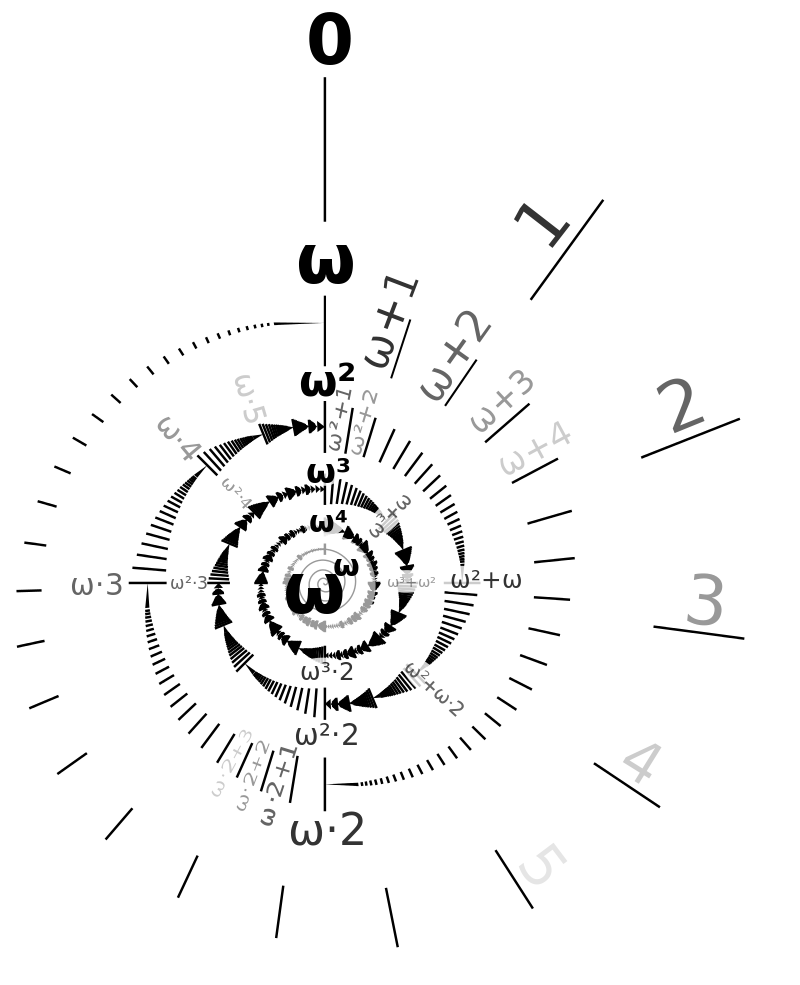
\includegraphics[width=43mm]{ordinal-spiral.png}
\caption{\url{https://commons.wikimedia.org/wiki/File:Omega-exp-omega-labeled.svg}}
\end{figure}

\subsection{Lecture 8}

\begin{lemma}\label{alt-def}
Let $\alpha$ and $\beta$ be distinct ordinals. If $\alpha \subset \beta$, then $\alpha \in \beta$.
\end{lemma}
\begin{proof}
Suppose that $\alpha \subsetneq \beta$. Then $\beta \setminus \alpha \ne \emptyset$. Let $\gamma = \min\{x \mid x \in \beta \setminus \alpha\}$. We claim that $\alpha = \gamma$, in which case $\alpha \in \beta$. 

\smallskip
Let $x \in \alpha$. Since $\left(\beta, \in\right)$ is a linear ordering and $\gamma \in \beta$, it follows that either $\gamma \in x$, $x= \gamma$, or $x \in \gamma$. In either of the the first two cases, $\gamma \in \alpha$, which is impossible. Hence $x \in \gamma$. This shows that $\alpha \subset \gamma$.  

\smallskip
 Conversely, let $x \in \gamma$. Since $\gamma \subset \beta$, we get $x \in \beta$. By our choice of $\gamma$, it follows that $x \in \alpha$. Hence $\gamma \subset \alpha$.
\end{proof}

\begin{lemma} \label{ord-wo}
$\left(\ord, \in\right)$ is a well-ordered class.
\end{lemma}
\begin{proof}
It is clear that $\in$ is set-like. Let $S \subset \ord$ be a nonempty subset. We must show that $S$ has a minimal element. Note that $\bigcap{S} \subset \alpha$ for every $\alpha \in S$. Therefore, $\left(\bigcap{S}, \in\right)$ is a  well-ordering as the restriction of a well-ordering. Now, suppose that $\beta \in \bigcap{S}$. Then $\beta \in \alpha$ for every $\alpha \in S$. By transitivity, for any $x\in \beta$, we have  $x \in \alpha$ for every $\alpha \in S$, so that $\beta \subset \bigcap{S}$. This implies that $\bigcap{S}$ is transitive. Hence $\bigcap{S}$ is an ordinal. By \cref{alt-def}, we see that $\bigcap{S}$ is minimal. 

\smallskip

It remains to show that $\ord$ is linearly ordered. By \cref{alt-def}, it suffices to show that if $\alpha$ and $\beta$ are ordinals, then either $\alpha \subset \beta$ or $\beta \subset \alpha$. Suppose, towards a contradiction, that  both $\alpha \not \subset \beta$ and $\beta \not \subset \alpha$. Our last paragraph shows that $\alpha \cap \beta$ is an ordinal, which must be a proper subset both of $\alpha$ and of $\beta$. \Cref{alt-def} implies that $\alpha \cap \beta \in \alpha$ and $\alpha \cap \beta \in \beta$. Hence $\alpha \cap \beta \in \alpha \cap \beta$, a contradiction. 
\end{proof}

\begin{corollary}
If $S$ is a nonempty set of ordinals, then  $\bigcap{S} = \min(S)$.
\end{corollary}

\begin{lemma}\label{PL}
Let $\left(W, <\right)$ be a woset. Suppose that for every $x\in W$, there is some ordinal $Z(x)$ such that $Z(x) \cong W_x$. Then $W$ is isomorphic to some ordinal. 
\end{lemma}
\begin{proof}
\Cref{non-iso} together with \cref{ord-wo} proves that such a $Z(x)$ must be unique. Therefore, $$A\coloneqq \{Z(x) \mid x \in W\}$$ is a set by $\mathsf{Rep}$. Note that $\left(A, \in\right)$ is a well-ordering. To see that $A$ is transitive, let $v\in A$. Then $v = Z(y)$ for some $y\in W$. Let $x\in Z(y)$. Then $$ x \cong X_{g_y^{-1}(x)} \cong Z(g^{-1}_y(x))    $$ where $g_y : W_y \overset{\cong}{\longrightarrow} Z(y)$.  This implies that $x = Z(g^{-1}_y(x))$ since both $x$ and $Z(g^{-1}_y(x))$ are ordinals. Thus, $x \in A$, so that $v\subset A$.

\smallskip

Define $f : W \to A$ by $f(x) = Z(x)$. 
\begin{claim} 
Let $x,y\in W$. Then $x <y \implies Z(x) \subsetneq Z(y)$. 
\end{claim}
\begin{proof}
Let $x<y$. Consider the isomorphism $g_y : W_y \to Z(y)$. We have that $$W_x = \left\{z\in W_y \mid  z < x\right\} = \left(W_y\right)_x.$$ Hence $g_y\restriction_{W_x}$ is an isomorphism from $W_x$ onto $Z(y)\restriction_{g_y(x)}$. It follows that $Z(y)\restriction_{g_y(x)} \cong Z(x)$, so that $$Z(x) = Z(y)\restriction_{g_y(x)} \subsetneq Z(y),$$ as desired. 
\end{proof}
By \cref{alt-def}, it follows that $f$ is order-preserving. Since $f$ is clearly surjective, it is an isomorphism.
\end{proof}

\begin{theorem} 
For any woset $\left(W, <\right)$, there is a unique ordinal $\alpha$ such that $W \cong \alpha$.
\end{theorem}
\begin{proof}
\Cref{non-iso} together with \cref{ord-wo} proves that such an $\alpha$ must be unique. We must prove that such an $\alpha$ exists.
\begin{claim}
For any $x\in W$, there is some ordinal $Z(x)$ such that $W_x \cong Z(x)$.
\end{claim}
\begin{proof}
Now, suppose, towards a contradiction, that the set $D\coloneqq \{ x\in W \mid W_x$ is not isomorphic to an ordinal$\}$ is nonempty.   Let $m = \min(D)$. Then for each $y< m$, there is some ordinal $Z(y)$ such that $\left(W_m\right)_y = W_y \cong Z(y)$.  By \cref{PL}, this implies that $W_m$ is isomorphic to some ordinal, contrary to our choice of $m$.
\end{proof}It follows from \cref{PL} that $W \cong \alpha$ for some ordinal $\alpha$.
\end{proof}

\subsection{Lecture 9}

\begin{lemma}[Transfinite induction]
Suppose that $C$ is a class of ordinals. Suppose that
\begin{enumerate}[label = (\alph*)]
\item $0\in C$,
\item $\alpha +1 \in C$ whenever $\alpha \in C$, and
\item for any nonzero limit $\lambda$, $\lambda \in C$ whenever $\left\{\beta \mid \beta < \lambda\right\} \subset C$. 
\end{enumerate}
Then $C = \ord$. 
\end{lemma}
\begin{proof}
Suppose, towards a contradiction, that $\ord \setminus C \ne \emptyset$. Let $m = \min(\ord \setminus C)$. It's easy to see that $ m$ is neither zero nor a successor. Hence $m$ is a nonzero limit. By condition (c), there must be some $\alpha < \lambda$ such that $\alpha \notin C$. Then $\alpha \in \ord \setminus C$, so that $m$ is not minimal, a contradiction. 
\end{proof}

\begin{note}
We can replace the condition ``$\alpha +1 \in C$ whenever $\alpha \in C$" with the condition ``$\alpha +1 \in C$ whenever $\left\{\beta \mid \beta \leq \alpha\right\} \subset C$."
\end{note}

\begin{theorem}[Transfinite recursion]
Let $\mathsf{Seq}$ denote the class $\left\{ f : \alpha \to x \mid \alpha \in \ord \land x\in V\right\}$ of all \textit{transfinite sequences}. For any class functional relation $G:\mathsf{Seq} \to V$, there exists a unique class function $F: \ord \to V$ such that $$ F(\alpha) =G(F\restriction_{\alpha})    $$ for every $\alpha \in \ord$.
\end{theorem}
\begin{proof}
We use transfinite induction to prove that there is a proper class $\langle f_{\alpha} \mid \alpha \in \ord \rangle$ (viewed as a sequence) such that for each $\alpha \in \ord$,  $f_{\alpha}$ is the unique function such that 
\begin{enumerate}[label=(\roman*)]
\item $\dom{f_{\alpha}} = \alpha$,
\item for any $\beta \in \alpha$, $f_{\alpha}(\beta)= G(f_{\alpha}\restriction_{\beta})$, and
\item for any $\beta \in \alpha$, $f_{\alpha}\restriction_{\beta} = f_{\beta}$.
\end{enumerate}
There are three cases to consider for our induction.
\begin{itemize}
\item Suppose that $\alpha = 0$. Then $f_{\alpha} \coloneqq \emptyset$ is the unique function satisfying all three conditions. 
\item Suppose that $\alpha = \beta +1$ and that there exists a unique $f_{\beta}$ satisfying all three conditions. Let
\[ 
f_{\beta+1}(\gamma) =
\begin{cases}
G(f_{\beta}) & \gamma = 	\beta
\\ f_{\beta}(\gamma) & \gamma < \beta
\end{cases}.
\] Let $\delta \in \beta +1$.  If $\delta = \beta$, then $f_{\beta+1}(\delta) = G(f_{\beta}) = G(f_{\beta+1}\restriction_{\beta}) = G(f_{\beta+1}\restriction_{\delta}) .$ If $\delta \in \beta$, then $f_{\beta+1}(\delta) = \underbrace{f_{\beta}(\delta) = G(f_{\beta}\restriction_{\delta})}_{\text{by induction}} = G(f_{\beta+1}\restriction_{\delta})$. 
Moreover, $f_{\beta +1}\restriction_{\beta} = f_{\beta}$, and $f_{\beta +1}\restriction_{\gamma} = f_{\beta}\restriction_{\gamma} = f_{\gamma}$ for any $\gamma \in \beta$ by induction. We have shown that $f_{\beta +1}$ satisfies all three properties. 

 It remains to show that $f_{\beta +1}$ is unique. Suppose that there is another function $g$ satisfying all three properties for $\beta +1$. Suppose, towards a contradiction, that the set $E\coloneqq \{\alpha  \in \beta +1 \mid g \ne f_{\beta +1}\}$ is nonempty. Let $m = \min(E)$. Then $g\restriction_m = f_{\beta +1}\restriction_m $, so that $$g(m) = G(g\restriction_m)  = G(f_{\beta +1}\restriction_m) = f_{\beta +1}(m),$$ a contradiction. It follows that $g = f_{\beta +1}$.
\item Suppose that $\alpha$ is a nonzero limit and that, for each $\beta \in \alpha$, there exists a unique $f_{\beta}$ satisfying all three conditions. Let $$f_{\alpha} =\bigcup_{\beta \in \alpha} f_{\beta}.$$ By applying $\mathsf{Rep}$ followed by $\mathsf{Union}$, we see that $f_{\alpha}$ is a set. By condition (iii) from our IH, we also see that $f_{\alpha}$ is a partial function on $\alpha$. In fact, since $\alpha$ is a limit, $f_{\alpha}$ has domain equal to $\alpha$. Hence $f_{\alpha}$ satisfies condition (i). Further, it is clear that $f_{\alpha}$ satisfies condition (iii). 

Let $\beta \in \alpha$. Note that $\beta +1 \in \alpha$. By applying our IH, we get
\begin{align*}
f_{\alpha}(\beta) & = f_{\beta +1}(\beta)  
\\ &  = G(f_{\beta +1}\restriction_{\beta}) 
\\ & = G(f_{\beta})  
\\ & = G(f_{\alpha}\restriction_{\beta}).
\end{align*}
This shows that $f_{\alpha}$ satisfies condition (ii). The fact that $f_{\alpha}$ is unique follows exactly as in our last case.
\end{itemize}$ $This completes our induction. Now, define $F: \ord \to V$ by $\alpha \mapsto G(f_{\alpha})$. This is clearly a class function. Also, if $\alpha \in \ord$, then $F\restriction_{\alpha} = \left\{(\beta, F(\beta)) \mid \beta \in \alpha\right\}$ is a set by $\mathsf{Rep}$ because  each $F(\beta)$ is a set. Note that $\dom{f_{\alpha}} = \alpha = \dom{F\restriction_{\alpha}}$ and that for any $\beta \in \alpha$,
$$  f_{\alpha}(\beta) = G(f_{\alpha}\restriction_{\beta}) =  G(f_{\beta})= F_{\alpha}(\beta)  .$$ Therefore, $f_{\alpha} = F\restriction_{\alpha}$, so that $F(\alpha) = G(F\restriction_{\alpha})$, as required. 

\smallskip

Let $F' : \ord \to V$ also have $F'(\alpha) = G(F'\restriction_{\alpha})$. Using transfinite induction, it is easy to check that $F'(\alpha) = F(\alpha)$ for any ordinal $\alpha$. Thus, $F$ is unique. 
\end{proof}


\subsection{Lecture 10}\label{Lecture10}


\begin{exercise}\label{ord-char}
Show that a set $x$ is an ordinal if and only if $x$ is transitive and every $y\in x$ is transitive. 
\end{exercise}

\begin{lemma}
If $\alpha$ is an ordinal and $x\in \alpha$, then $x$ is an ordinal. 
\end{lemma}
\begin{proof}
This follows from the ($\Longrightarrow$) direction of \cref{ord-char}.
\end{proof}

\begin{corollary}\label{LC}
If $X$ is a nonempty set of ordinals, then $\bigcup{X}$ is an ordinal and $\sup(X) = \bigcup{X}$.
\end{corollary}

\begin{corollary}[Burali-Forti]\label{B-F}
$\ord$ is a proper class.
\end{corollary}
\begin{proof}
Otherwise, $\sup{\ord}$ and $\sup{\ord}+1$ are ordinals by \cref{LC}, in which case $$\sup{\ord} < \sup{\ord} +1 \leq \sup{\ord},$$ a contradiction. 
 \end{proof}

\begin{definition}
 An ordinal $\kappa$ is a \textit{cardinal (number)} (written as $\card(\kappa)$) if for every ordinal $\lambda < \kappa$, $\kappa \not \sim \lambda$.
\end{definition}

\begin{exmp} $ $
The finite cardinals are precisely the finite ordinals. In addition, $\omega$ is an infinite cardinal.
\end{exmp}

\begin{note}
Every infinite cardinal is a nonzero limit ordinal. 
\end{note}

\begin{definition}
Let $X$ and $Y$ be sets. 
\begin{enumerate}
\item Let $\left\lvert{X}\right\rvert \leq \left\lvert{Y}\right\rvert$ if there is an injection from $X$ into $Y$. 
\item Let $\left\lvert{X}\right\rvert<\left\lvert{Y}\right\rvert$ if $\left\lvert{X}\right\rvert \leq \left\lvert{Y}\right\rvert$ but $\left\lvert{Y}\right\rvert \not \leq \left\lvert{X}\right\rvert$.
\end{enumerate}
\end{definition}

\begin{theorem}[Cantor-Schr\"oder-Bernstein]\label{CSB}
If $\left\lvert{X}\right\rvert\leq \left\lvert{Y}\right\rvert$ and $\left\lvert{Y}\right\rvert\leq \left\lvert{X}\right\rvert$, then $\left\lvert{X}\right\rvert = \left\lvert{Y}\right\rvert$.
\end{theorem}


\begin{theorem}[Cantor]
$\left\lvert{X}\right\rvert < \left\lvert{\P(X)}\right\rvert$.
\end{theorem}
\begin{proof}
It's clear that $\left\lvert{X}\right\rvert \leq \left\lvert{\P(X)}\right\rvert$. Let $f: X \to \P(X)$. Consider the set $$Z\coloneqq \{x\in X \mid x \notin f(x)    \} .$$ If $Z= f(y)$ for some $y\in X$, then $y\in Z \iff y\notin Z$, which is false. Thus, $Z\notin \im{f}$. This shows that there is no surjection (and hence no bijection) from $X$ onto $\P(X)$. By \cref{CSB}, it follows that   $\left\lvert{\P(X)}\right\rvert \not \leq \left\lvert{X}\right\rvert$, so that $\left\lvert{X}\right\rvert < \left\lvert{\P(X)}\right\rvert$.
\end{proof}


\begin{remark}
Recall that $\R \sim \P(\omega)$. The continuum hypothesis asserts that there is no set $X$ such that $\left\lvert{\omega}\right\rvert < \left\lvert{X}\right\rvert < \left\lvert{\P(\omega)}\right\rvert$.
\end{remark}

\begin{definition}
For any set $X$, let $H(X)$ denote the least ordinal $\alpha$  such that $\alpha \not \sim X$. We call $H(X)$ the \textit{Hartogs number of $X$}. 
\end{definition}


\begin{theorem}
For every cardinal $\kappa$, there is some cardinal $\lambda > \kappa$.
\end{theorem}
\begin{proof}
Suppose that $H(\kappa)$ exists. Then $\kappa \sim \beta$ for some $ \beta \in H(\kappa) $, so that $\left\lvert{\kappa}\right\rvert \leq \left\lvert{H(\kappa)}\right\rvert$. But clearly  $\left\lvert{\kappa}\right\rvert \ne \left\lvert{H(\kappa)}\right\rvert$. Therefore, $\left\lvert{\kappa}\right\rvert < \left\lvert{H(\kappa)}\right\rvert$, which means that it suffices to show that $H(\kappa)$, in fact, exists.

\smallskip
 Note that the class $D$ of all well-orderings of $\kappa$ is a subclass of the set $\P(\kappa \times \kappa)$. Hence $D$ is a set by $\mathsf{Sep}$. If  $H(\kappa)$ does not exist, then we get an injective class function $F: \ord \to D$. In this case, $\im{F^{-1}} = \ord$ is a set by $\mathsf{Rep}$, a contradiction. Thus, $H(\kappa)$ exists. 
\end{proof}

\begin{note}
Our proof shows that $H(X)$ exists for any $X$ in $\zf$.
\end{note}

\begin{notation}
If $\kappa$ is a cardinal, then let $\kappa^+$ denote the least cardinal greater than $\kappa$. 
\end{notation}


\begin{corollary}
The class $C$ of all cardinals is a proper class.
\end{corollary}
\begin{proof}
For any ordinal $\alpha$, consider the cardinal $\kappa = \min\{\beta \in \ord \mid \beta \sim \alpha\}$. By Cantor-Schr\"oder-Bernstein, it's easy to check that $\alpha < \kappa^+$. Therefore,  if $C$ is a set, then $\bigcup{C}$ is a set and equals $\ord$, a contradiction. Hence $C$ is a proper class.
\end{proof}

\begin{definition}
By transfinite recursion, define the sequence
\begin{align*}
\aleph_0 & = \omega
\\ \aleph_{\alpha +1} & =\aleph_{\alpha}^+
\\ \aleph_{\lambda} & = \bigcup_{\beta \in \lambda} \aleph_{\beta} \text{ when }\lambda >0 \text{ is a limit.}
\end{align*}   The symbol $\omega_{\alpha}$ means the same thing as $\aleph_{\alpha}$.
\end{definition}

\begin{lemma}
If $\lambda >0$ is a limit ordinal, then $\card(\aleph_{\lambda})$.
\end{lemma}
\begin{proof}
Suppose, towards a contradiction, that there exist  an $x\in \aleph_{\lambda}$ and a bijection $f: x \to \aleph_{\lambda}$. Then $x\in \aleph_{\beta}$ for some successor $\beta \in \lambda$. It follows that $$\left\lvert{ \aleph_{\lambda}  }\right\rvert = \left\lvert{ x  }\right\rvert \leq \left\lvert{  \aleph_{\beta} }\right\rvert \leq \left\lvert{ \aleph_{\lambda}  }\right\rvert .$$ Hence $ \aleph_{\beta} \sim x$. But we know that $\aleph_{\beta} $ is a cardinal, a contradiction. 
\end{proof}

\section{The axiom of choice}

\begin{definition}[The axiom of choice ($\ac$)]
Let $I$ be a set and $C = \left\{A_i  \right\}_{i\in I}$ where each $A_i$ is nonempty. Then there is a function $f : I \to \bigcup{C}$ such that $f(i) \in A_i$ for each $i\in I$. (Such an $f$ is called a \textit{choice function}.)
\end{definition}


\begin{notation}
Let $\zfc$ denote the theory $\zf + \ac$.
\end{notation}

\begin{definition}[Zermelo's well-ordering principle ($\mathsf{WOP}$)]
For any set $x$, there is some cardinal $\lambda$ such that $x \sim \lambda$.
\end{definition}

\begin{theorem}\label{AW}
$\ac \iff \mathsf{WOP}$.
\end{theorem}

\begin{definition}{$(\zfc)$}
Let $X$ be a set, The \textit{cardinality of $X$} is the cardinal number $$\left\lvert{X}\right\rvert \coloneqq \min\{\alpha \in \ord \mid \alpha \sim X\}.$$
\end{definition}

\begin{remark}\label{LR} $ $
\begin{enumerate}
\item One can show that $\zf \nvDash \underbrace{\forall X\forall Y(\left\lvert{X}\right\rvert \leq \left\lvert{Y}\right\rvert \vee \left\lvert{Y}\right\rvert \leq \left\lvert{X}\right\rvert)}_{\psi}$. In fact,  $\ac$ is equivalent to the sentence $\psi$. In particular, $\ac$ is independent of $\zf$.
\item Let $\varphi$ denote the sentence ``Every surjection has a right inverse."  Then $\zf \nvDash \varphi$, whereas  $\zfc \models \varphi$. Since every right inverse is injective, the following assertion is also provable in $\zfc$: If there exists a surjection of $X$ onto $Y$, then $\left\lvert{Y}\right\rvert \leq \left\lvert{X}\right\rvert$. 
\item We can, however, prove in $\zf$ that every injection has a left inverse and that every left inverse is surjective. Therefore, in $\zf$, if $\left\lvert{Y}\right\rvert \leq \left\lvert{X}\right\rvert$, then there is a surjection of $X$ onto $Y$. It follows that, in $\zfc$, $\left\lvert{Y}\right\rvert \leq \left\lvert{X}\right\rvert$ if and only if there is a surjection of $X$ onto $Y$.
\end{enumerate}
\end{remark}

\begin{note}[Linear ordering of cardinals]
\begin{enumerate}
\item Consider the binary relation $< $ on the class of all cardinal numbers where $\left\lvert{X}\right\rvert < \left\lvert{Y}\right\rvert$ if there is an injection from $X$ intro $Y$ but $\left\lvert{X}\right\rvert \ne \left\lvert{Y}\right\rvert$. In light of the Cantor-Schr\"oder-Bernstein, we see that $<$ is a partial ordering. By \cref{LR}, we see that $<$ is actually a linear ordering in $\zfc$. 
\item In $\zfc$, if $\lambda$ is an infinite cardinal, then $\lambda = \aleph_{\alpha}$ for some ordinal $\alpha$. In this case, we get a transfinite enumeration of class of all cardinals
\[
0 < 1 < 2 < 3 < \cdots < \aleph_0 < \aleph_1 < \aleph_2 < \aleph_3 <  \cdots < \aleph_{\omega} < \cdots
.\]
\end{enumerate}
\end{note}

\begin{definition}[Cardinal arithmetic (in $\zfc$)] Let $\kappa$ and $\lambda$ be cardinals. Define cardinal addition, multiplication, and exponentiation, respectively, as follows.
\begin{enumerate}
\item $\kappa + \lambda = \left\lvert{\kappa \coprod \lambda}\right\rvert$.
\item $\kappa \cdot \lambda = \left\lvert{\kappa \times \lambda}\right\rvert $.
\item $\kappa^{\lambda} = \left\lvert{\{f \mid f : \lambda \to \kappa \}}\right\rvert$.
\end{enumerate} 
\end{definition}

\begin{note}
For any ordinal $\alpha$,  the lexicographic ordering of $\alpha \times \alpha$ is a well-ordering. Hence we do not need the axiom of choice for our definition of cardinal multiplication. 
\end{note}

\begin{lemma}{$(\zf)$}
$\aleph_{\alpha} \cdot \aleph_{\alpha} = \aleph_{\alpha}$ for any ordinal $\alpha$.
\end{lemma}
\begin{proof} 
Consider the binary class relation $\lhd$ on $\ord \times \ord$ where $\left(\alpha, \beta\right)\lhd \left(\gamma, \delta\right)$ if at least one of the following conditions holds.
\begin{itemize}
\item  $\max\{\alpha, \beta\} <\max\{\gamma, \delta\}$.
\item $\max\{\alpha, \beta\} = \max\{\gamma, \delta\}$ and $\alpha < \delta$.
\item $\max\{\alpha, \beta\} = \max\{\gamma, \delta\}$ and $\alpha =\delta$ and $\beta < \delta$. 
\end{itemize}$ $It is straightforward to check that $\lhd$ is a well-ordering. Now, define the class function $\Gamma : \ord \times \ord \to \ord$ by $\gamma(\alpha, \beta) = \delta$ where $\delta$ is the unique ordinal isomorphic to the initial segment $\left(\ord \times \ord\right)_{(\alpha, \beta)}$. It is easy to see that $\Gamma$ is injective. Thus, it suffices to show that $$\Gamma(\omega_{\alpha} \times \omega_{\alpha}) = \omega_{\alpha}$$ for each ordinal $\alpha$. 

\smallskip

Note that for any $\left(n,m\right) \in \omega \times \omega$, $$ \Gamma(n,m) = 
m(n+1).$$ Hence $\omega =\Gamma(\omega \times \omega)$, as desired.  

\smallskip
 Suppose, towards a contradiction, that the class $E\coloneqq \{x >0 \mid \Gamma(\omega_{x} \times \omega_{x}) \ne \omega_{x}\}$ of ordinals is nonempty. Let $\beta = \min( E )$ . Then \hl{$\Gamma(\gamma, \delta) = \omega_{\beta}$} for some $\gamma, \delta \in \omega_{\beta}$. Since $\omega_{\beta}$ is a limit, we can find some $\eta \in \omega_{\beta}$ such that $\gamma,\delta \in \eta$. Note that $\left(\gamma, \delta\right) \in \eta \times \eta$. Since $\eta \times \eta = \left(\ord \times \ord\right)_{(0, \eta)}$, it follows that $$\Gamma(\eta \times \eta) \supset \underbrace{\Gamma(\{\left(x,y\right) \mid \left(x,y\right) \lhd \left(\gamma, \delta\right)\})}_{\text{transitive}} \supset \omega_{\beta}. $$ This implies that $\left\lvert{\aleph_{\beta}}\right\rvert \leq \left\lvert{\eta \times \eta}\right\rvert$. But $$\left\lvert{\eta \times \eta}\right\rvert=  \left\lvert{\left\lvert{\eta}\right\rvert \times \left\lvert{\eta}\right\rvert}\right\rvert = \left\lvert{\eta}\right\rvert < \aleph_{\beta}   ,$$ a contradiction. 
\end{proof}

\begin{corollary}{$(\zfc)$}
Let $\kappa$ and $\lambda$ be infinite cardinals.
Then $$\kappa \cdot \lambda = \kappa + \lambda = \max\{\kappa, \lambda\}.$$
\end{corollary}

\subsection{Lecture 11}

\begin{remark}
If $\U$ denotes the universe of all sets, then $\zf \setminus \{\mathsf{Reg}\} \vdash \mathsf{Reg} \leftrightarrow \U = V$.
\end{remark}$ $
We now prove a theorem stated in \cref{Lecture10}.

\begin{proof}{\textbf{($\ac \iff \mathsf{WOP}$)}}$ $\\ 
($\Longleftarrow$) Let $I$ be any set and let $C\coloneqq \{A_i\}_{i\in I}$ be a collection of nonempty sets. By  $\mathsf{Union}$, we see that $\bigcup C$ is a set. By $\mathsf{WOP}$, there exists a well-ordering $<$ on $\bigcup C$. Note that each $A_i$ is a nonempty subset of $\bigcup C$. Thus, $A_i$ contains a least element $a_i$. Now, define $f: I \rightarrow \bigcup C$ by $f(i)=a_i$. As long as $f$ is well-defined, it is a choice function. To show that it is well-defined, it suffices to show that the $a_i$ are unique. Suppose that both $a_i$ and $b_i$ are minimal elements of $A_i$. Note  that $<$ is a linear ordering of $C$. Thus, either $a_i \leq b_i$ or $b_i\leq a_i$. But both are minimal, so that, in either case, $a_i=b_i$. This shows that $f$ is well-defined.

\smallskip

($\Longrightarrow$) Let $X$ be a set. Let $E = \P(X) \setminus \{\emptyset\}$, which is a collection of nonempty sets. By $\ac$, there is some choice function $f : E \to \bigcup{E}$.  By transfinite recursion, we can define a sequence $F : \ord \to V$ by 
$$ F(\alpha) = f(X \setminus \{F(\beta) \mid \beta \in \alpha \})   .$$ Since $f$ is a choice function, we have that $F(\alpha) \notin \{F(\beta) \mid \beta \in \alpha\}$ whenever $\left\{F(\beta) \mid \beta \in \alpha\right\} \ne X$. Hence if there is no $\delta \in \ord$ such that $\left\{F(\gamma) \mid \gamma \in \delta\right\} =X$, then $F$ is injective. But, in this case, $\im{F^{-1}} = \ord$ is a set by $\mathsf{Rep}$, a contradiction. Therefore, there exists a least such $\delta$. Then $F\restriction_{\delta}$ is a bijection from $\delta$ onto $X$.
\end{proof}

\begin{definition}
Let $\left(P, <\right)$ be a partially ordered set. A \textit{chain in $P$} is a nonempty subset $X\subset P$ such that $\left(X, <\restriction_X\right)$ is a linear ordering. 
\end{definition}

\begin{definition}[Zorn's lemma ($\mathsf{Zorn}$)]
If $\left(P, <\right)$ is a nonempty poset and every chain in $P$ has an upper bound in $P$, then $P$ has a maximal element. 
\end{definition}

\begin{lemma}
$\mathsf{WOP} \implies \mathsf{Zorn}$.
\end{lemma}
\begin{proof} Let $\left(P, <_P\right)$ be a nonempty poset such that every chain in $P$ has an upper bound in $P$. By assumption, we have a bijection $f : \lambda \to P$ for some cardinal $\lambda$. We see that $\lambda >0$ for otherwise $P = \emptyset$. Note that $P = \left\{f(\delta) \mid \delta \in \lambda\right\}$. By transfinite recursion, define $F: \ord \to \lambda +1$ by
\[
F(\alpha) = \begin{cases}
\min\{\gamma \in \lambda \mid \beta \in \alpha \rightarrow f(F(\beta)) <_P f(\gamma)\} &\{\gamma \in \lambda \mid \beta \in \alpha \rightarrow f(F(\beta)) <_P f(\gamma)\} \ne \emptyset
\\ \lambda & \text{otherwise}
\end{cases}.
\]  Note that $\alpha_1 < \alpha _2 \implies F(\alpha_1) <_P F(\alpha_2)$ provided that $ F(\alpha_1),  F(\alpha_2) \in \lambda$, in which case $\im{F^{-1}}= \ord$ is a set by $\mathsf{Rep}$, a contradiction. 

\smallskip
Therefore, there is some smallest nonzero $\delta \in \ord$ such that $F(\delta) = \lambda$. This implies that $\left\{f(F(\beta)) \mid \beta \in \delta\right\}$ is a chain in $P$. If $\delta$ is a limit, then $P$ has no upper bound, a contradiction. Thus, $\delta = \eta + 1$ for some ordinal $\eta$. Suppose that $f(F(\eta))$ is not maximal in $P$. Then there is some least $\tau \in \lambda$ such that $f(F(\eta)) <_P f(\tau)$. But this means $$\lambda = F(\delta) = \tau \in \lambda,$$ a contradiction. It follows that $f(F(\eta))$ is a maximal element.  
\end{proof}

\begin{prop}
$\mathsf{Zorn} \implies \mathsf{WOP}$.
\end{prop}

\begin{corollary}
$\ac \iff \mathsf{WOP} \iff \mathsf{Zorn}$.
\end{corollary}

\begin{definition} Let $S$ be a set. Let $F$ be a subset of $\P(S)$. We say that $F$  is a \textit{filter on $S$} if
\begin{enumerate}[label=(\alph*)]
\item $F\ne \emptyset$,
\item $\emptyset \notin F$,
\item if $X \in F$ and $X \subset Y$, then $Y \in F$, and
\item $X,Y \in F \implies X \cap Y \in F$.
\end{enumerate}
\end{definition}

\begin{exmp}
The \textit{Fr\'echet filter} on $S$ is the set of all cofinite sets in $S$.
\end{exmp}

\begin{definition}  Let $F$ be a filter on $S$.
\begin{enumerate}
\item We say that $F$ is an \textit{ultrafilter} if for any $X \in \P(S)$, either $X \in F$ or $\left(S \setminus X\right) \in F$.
\item If $F$ is an ultrafilter, then we say that $F$ is \textit{nonprincipal} if it contains the Fr\'echet filter on $S$.
\end{enumerate} 
\end{definition}

\begin{remark}
Let $F$ be an ultrafilter on $S$. Define $\mu : \P(S) \to \left\{0, 1\right\}$ by $$\mu(A) =\begin{cases} 1 & A \in F \\ 0 & A \notin F \end{cases} .$$ Then $\mu$ is a measure on $S$ so long as we substitute the condition of finite additivity for that of countable additivity.    
\end{remark}

\begin{definition}
A subset $G\subset \P(S)$ has the \textit{finite intersection property} (FIP) if $$Z_1, \ldots, Z_k \in G \implies Z_1 \cap \cdots \cap Z_k \ne \emptyset.$$
\end{definition}

\begin{lemma}\label{FIP}
If $G\subset \P(S)$ has FIP, then there is some filter $H$ on $S$ such that $H\supset G$.
\end{lemma}
\begin{proof}
Take $H = \left\{W\subset S \mid \text{ there exist a } k\in \N \text{ and } Z_1, \ldots, Z_k \in G\text{ such that } Z_1 \cap \cdots \cap Z_k \subset W\right\}$.
\end{proof}

\begin{theorem}
Every filter $E$ on $S$ can be extended to an ultrafilter.
\end{theorem}
\begin{proof}
Let $\mathcal{F} = \left\{F \subset \P(S) \mid F \text{ is a filter on }S,\  F\supset E\right\}$. Then $\left(\mathcal{F}, \subset\right)$ is a poset with $E\in \mathcal{F}$. 
\begin{claim}
 A filter $F\subset \P(S)$ is an ultrafilter if and only if it is maximal in $\mathcal{F}$.
\end{claim}
\begin{proof}
It is clear that if $F$ is an ultrafilter, then it is maximal. For the converse, suppose that $F$ is not an ultrafilter. Then there is some $X\in \P(S)$ such that both $X \notin F$ and $\left(S\setminus X\right) \notin F$. We must show that $F$ is not maximal in $\mathcal{F}$. 
Note that for any $Y \in F$, the intersection $X \cap Y$ is nonempty. Therefore, $F \cup \left\{X\right\}$ has FIP. By \cref{FIP}, $F \cup \left\{X\right\}$ can be extended to a filter $H$ on $S$. But $H \supsetneq F \supset E$, so that $F$ is not maximal in $\mathcal{F}$.
\end{proof}
Thus, it suffices to show that $\mathcal{F}$ has some maximal element. Let $C$ be a chain in $\mathcal{F}$. It is easy to check that $\bigcup{C}$ is an upper bound of $C$ in $\mathcal{F}$. It follows from $\mathsf{Zorn}$ that $\mathcal{F}$ has some maximal element. 
\end{proof}

\begin{corollary}
There exists a nonprincipal ultrafilter. 
\end{corollary}

\begin{definition} Let $\kappa$ be an infinite cardinal.
\begin{enumerate}
\item A filter $F\subset \P(S)$ is \textit{$\kappa$-complete} if every subset $X\subset F$ with $\left\lvert{X}\right\rvert < \kappa$ satisfies $\bigcap{X} \in F$.
\item We say that $\kappa$ is \textit{measurable} if $\kappa > \omega$ and there exists a nonprincipal $\kappa$-complete ultrafilter on $\kappa$. 
\end{enumerate}
\end{definition}

\begin{definition}
A filter $F\subset \P(S)$ is \textit{$\sigma$-complete} if for any countable set $C$ of elements of $F$, we have $\bigcap{C} \in F$.
\end{definition}

\begin{prop}
The least cardinal $\kappa$  with a $\sigma$-complete nonprincipal ultrafilter is measurable. 
\end{prop}

\subsection{Lecture 12}

\begin{definition}
Let $\alpha$ and $\beta$ be nonzero limit ordinals. 
\begin{enumerate}
\item Let $f: \alpha \to \beta$. We say that $f$ is \textit{cofinal in $\beta$}, written as \textit{$f : \alpha \xrightarrow{\text{cofinally}} \beta$}, if $\sup(\im{f}) = \beta$. 
\item The \textit{cofinality $\cf(\alpha)$  of $\alpha$} is the least ordinal $\gamma$ for which there exists a cofinal map $f: \gamma \to \alpha$.
\end{enumerate}
\end{definition}

\begin{exmp} $ $
\begin{enumerate}
\item $\cf(\aleph_{\alpha}) = \cf(\alpha)$ for any limit ordinal $\alpha >0$.
\item $\cf(\omega) =  \omega$.
\end{enumerate}
\end{exmp}


\begin{definition} Let $\kappa$ be a cardinal.
\begin{enumerate}
\item $\kappa$ is \textit{regular} if $\cf(\kappa) = \kappa$.
\item $\kappa$ is \textit{singular} if it is not regular.
\item $\kappa$ is a \textit{limit (cardinal)} if $\lambda <\kappa \implies \lambda^+ < \kappa$.
\item $\kappa$ is a \textit{strong limit (cardinal)} if $\lambda < \kappa \implies 2^{\lambda} < \kappa$.
\item $\kappa$ is \textit{weakly inaccessible}  if it is an uncountable  regular limit.
\item $\kappa$ is \textit{(strongly) inaccessible} if it is an uncountable regular strong limit.
\end{enumerate} 
\end{definition}

\begin{note}
We can prove in $\zfc$ than any infinite successor cardinal $\kappa^+$ is regular. Indeed, since $\kappa^+$ is a limit ordinal, the identity function $\kappa^+ \to \kappa^+$ is cofinal in $\kappa^+$. If $\alpha < \kappa^+$ and $f : \alpha \to \kappa^+$ is a function, then $\left\lvert{f(\eta)}\right\rvert \leq \kappa$ for any $\eta < \alpha$. In this case, we thus have that
\begin{align*}
\left\lvert{\sup(\im(f))}\right\rvert & = \left\lvert{\bigcup_{\eta < \alpha}f(\eta)}\right\rvert
\\ & = \left\lvert{\alpha}\right\rvert \cdot \sup\left\{\left\lvert{f(\eta)}\right\rvert \mid \eta < \alpha\right\}
\\ & \leq \kappa \cdot \kappa
\\ & = \kappa
.\end{align*} This proves that  $f$ is \emph{not} cofinal in $\kappa^+$, so that $\cf(\kappa^+) = \kappa^+$.
\end{note}

\begin{prop} 
 If $\kappa$ is measurable, then $\kappa$ is strongly inaccessible and $\left\lvert{\{\lambda < \kappa \mid \lambda \text{ is inaccessible}\}}\right\rvert = \kappa$.
\end{prop}

\begin{remark} $ $
\begin{enumerate}
\item $\zf \nvDash ``\aleph_1 \text{ is regular}"$. In fact, in $\zf$, we can prove that there is some $f: \omega \to \aleph_1$ such that $\sup(\im{f}) = \aleph_1$, so that $\aleph_1 = \bigcup_{n \in \omega} f(n)$ even though each $f(n)$ is countable. 
\item If $\kappa$ is a strongly inaccessible cardinal, then $V_{\kappa} \models \zfc$.
\item  Let $\wi(\kappa)$ denote the assertion that $\kappa$ is a weakly inaccessible cardinal. It is known that $$\zfc \nvDash \exists{\kappa}(\wi(\kappa)).$$ Moreover, if $\con(\zfc + \exists{\kappa}(\wi(\kappa)))$ where $\con(T)$ means that the theory $T$ is consistent, then $\con(\zfc + \wi(2^{\aleph_0}))$.     . 
\end{enumerate}
\end{remark}

\begin{lemma}\label{card-prop}
For any $X$, we have $\left\lvert{\bigcup{X}}\right\rvert \leq \lambda \cdot \kappa$ where $\lambda$ denotes $\left\lvert{X}\right\rvert $ and $\kappa$ denotes $\sup\{\left\lvert{y}\right\rvert : y\in x\}$.
\end{lemma}
\begin{proof}
We can write $X=\left\{X_{\alpha} \mid \alpha <\lambda\right\}$. For each $\alpha <\lambda$, we have that $\kappa_{\alpha} \coloneqq \left\lvert{X_{\alpha}}\right\rvert \leq \kappa$. Therefore, we can also write $X_{\alpha} = \left\{x_{\alpha{\beta}} \mid \beta < \kappa_{\alpha}\right\}$. It follows that $$\bigcup{X} =\left\{ x_{\alpha{\beta}} \mid \alpha <\lambda, \ \beta < \kappa_{\alpha}\right\},   $$ which has cardinality at most $\left\lvert{\lambda \times \kappa}\right\rvert$.
\end{proof}

\begin{corollary}
A countable union of countable sets is countable.
\end{corollary}
\begin{proof}
Apply \cref{card-prop} with $\lambda =\omega$ and $\kappa = \omega$. Since $\omega \times \omega$ is countable, we're done.
\end{proof}

\begin{lemma}\label{PL'}
$\cf(\alpha)$ is a cardinal for any limit ordinal $\alpha >0$.
\end{lemma}
\begin{proof}
We can find a cofinal map $g: \cf(\alpha) \to \alpha$. Suppose, towards a contradiction, that $\cf(\alpha)$  is not a cardinal. Then there exist a $\delta \in \cf(\alpha)$  and a bijection $f: \delta \to \cf(\alpha)$. Then $\sup(\im{g\circ f}) = \sup(\im{g}) = \alpha $, so that $g \circ f$ is a cofinal map. This contradicts the minimality of $\cf(\alpha)$. 
\end{proof}

\begin{theorem}
For any infinite cardinal $\kappa$, $\kappa^+$ is regular. 
\end{theorem}
\begin{proof}
Note that $\cf(\alpha)\leq \alpha$ for any $\alpha$ since $\id_{\alpha}$ is a cofinal map. Thus, it suffices to show $\cf(\kappa^+) \geq \kappa^+$. 
\begin{claim}
If $\lambda \leq \kappa$, then $\cf(\kappa^+) > \lambda$. 
\end{claim}
\begin{proof}
Suppose, towards a contradiction, that $\cf(\kappa^+) \leq \lambda$ for some $\lambda \leq \kappa$. Then there is some $\eta \leq \lambda$ such that $$\kappa^+ = \bigcup{\left\{\alpha_i \mid i <\eta \right\}}$$ for some $\alpha_i \in \kappa^+$. Note that $\left\lvert{\alpha_i}\right\rvert \leq \kappa$ for each $i$ and that $\left\lvert{\eta}\right\rvert \leq \kappa$. By \cref{card-prop}, it follows $\kappa^+ \leq \kappa \cdot \kappa = \kappa$, a contradiction.  
\end{proof}But $\cf(\kappa^+)$ is a cardinal  by \cref{PL'}. Hence $\cf(\kappa^+) \geq \kappa^+$.
\end{proof}


\begin{definition} Let $I$ be a set. Consider any collection of sets $\left\{X_i\right\}_{i\in I}$ indexed by $I$.
The \textit{infinite sum of the $X_i$} is $\sum_{i\in I} X_i \coloneqq \coprod_{i\in I} X_i$. Let $\iota_i : X_i \to \sum_{i\in I} X_i $ denote the canonical inclusion. 
\end{definition}

\begin{theorem}[K\"onig]
If $\left\lvert{X_i}\right\rvert < \left\lvert{Y_i}\right\rvert$ for each $i \in I$, then $\left\lvert{\sum_{i\in I} X_i}\right\rvert < \left\lvert{\prod_{i\in I} Y_i}\right\rvert$.
\end{theorem}
\begin{proof}
We must show that $\left\lvert{\sum_{i\in I} X_i}\right\rvert \not \geq \left\lvert{\prod_{i\in I} Y_i}\right\rvert$. Suppose, to the contrary, that there is some surjection $f: \sum_{i\in I} X_i \to \prod_{i\in I} Y_i$. Since $\left\lvert{X_i}\right\rvert < \left\lvert{Y_i}\right\rvert$ for each $i\in I$ by hypothesis, the function $$f_i \coloneqq \pi_i \circ f \circ \iota_i: X_i \to Y_i$$ cannot be surjective where $\pi_i$ denotes the $i$-th projection map. For each $i$, we can thus choose some $y_i$ such that $y_i \notin \im{f_i}$. Since $f$ is surjective, there is some $x\in \sum_{i\in I} X_i $ such that $f(x) = \left(y_i\right)_{i\in I}$. But $x\in X_j$ for some $j\in I$, so that $y_j = f_j(x)$. This contradicts the fact that $y_j \notin \im{f_j}$. 
\end{proof}

\begin{corollary}
For any infinite cardinal $\kappa$, $\kappa< \cf(2^{\kappa})$.
\end{corollary}
\begin{proof}
Suppose, towards a contradiction, that there exist an $\eta \leq \kappa$ and a  sequence $\langle \alpha_i \mid i < \eta \rangle$ in $2^{\kappa}$ such that $$ \sup\{\alpha_i \mid i <\eta\} = 2^{\kappa}.$$ Then we get 
\begin{align*}    
2^{\kappa}  = \left(2^{\kappa}\right)^{\kappa} 
&  \geq  \left\lvert{ \prod_{i < \eta} 2^{\kappa}}\right\rvert 
> \left\lvert{\sum_{i < \eta} \alpha_i}\right\rvert
\\ & \geq \left\lvert{\sup\{\alpha_i \mid i <\eta\}}\right\rvert 
= 2^{\kappa}
,
\end{align*}  a contradiction. 
\end{proof}

\section{Relativization}

\subsection{Lecture 13}


\begin{lemma}\label{cum}
For any ordinal $\alpha$, $V_{\alpha}$ is transitive and $V_{\beta} \subset V_{\alpha}$ for every $\beta \leq \alpha$. 
\end{lemma}
\begin{proof}
Note that if a set $x$ is transitive, then  $\P(x)$ is transitive and $x\subset \P(x)$. In light of this, it's easy to use transfinite induction to complete our proof.
\end{proof}

\begin{corollary}
Let $x$ be a set. If every $y\in x$ belongs to $V$, then $x$ belongs to $V$. 
\end{corollary}
\begin{proof}
Using \cref{cum}, we have that $\bigcup{x} \in V$. Thus, $\bigcup{x}\subset V_{\beta}$ for some $\beta \in \ord$. This implies that $y \subset V_{\beta}$ for each $y\in x$. Hence $x\subset \P(V_{\beta}) = V_{\beta +1}$, so that $x \in \P(V_{\beta +1}) = V_{\beta +2}$.
\end{proof}

\begin{definition}
Let $x$ be a set. The \textit{transitive closure $\tc(x)$ of $x$} is defined recursively by
\begin{align*}
x_0 & = x
 \\ x_{n+1} & = \bigcup {x_n}
 \\ \tc(x) & = \bigcup_{n\in \omega} x_n.
\end{align*}
\end{definition}

\begin{note}
For any $x$, $\tc(x)$ is the smallest transitive set containing $x$, i.e., $$\tc(x) = \bigcap{\left\{y\supset x \mid y \text{ is a transitive set}\right\}}.$$
\end{note}

\begin{lemma}[Regularity for classes]\label{reg}
Let $C$ be a nonempty class. Then there is some $x\in C$ such that if $y\in C$, then $y \notin x$. In other words, $C$ has some $\in$-minimal element.
\end{lemma}
\begin{proof}
By assumption, there is some $u\in C$. Let $e = \left\{ x\in C \mid x \in \tc(u)\right\}$, which is a set by $\mathsf{Sep}$. If $e = \emptyset$, then there is no element of $C \cap u$, in which case $u$ is minimal in $C$. If $e\ne \emptyset$, then there is some $\in$-minimal element $m$ of $e$. In this case, no element $n$ of $m$ can belong to $C$. For otherwise $n\in m\subset \tc(u)$ and $n \in C$, so that $n \in e$, contrary to our choice of $m$. It follows that $m$ is minimal in $C$.
\end{proof}

\begin{definition}
The \textit{rank $\rnk(x)$ of a set $x$} is the least ordinal $\alpha$ such that $x\in V_{\alpha +1}$.
\end{definition}

\begin{lemma}
In $\zf$, every set is in $V$. In other words, $\zf \vdash \forall x(V(x))$.
\end{lemma}
\begin{proof}
Suppose, towards a contradiction, that there is some $z$ such that $\neg{V(z)}$. By \cref{reg}, there is some $\in$-minimal such set $m$. Then we have a functional relation $\rnk :  m \to \ord$. Hence $\im{\rnk}$ is a set, and we can form the set $\beta \coloneqq \sup(\im{\rnk})$, which is an ordinal. If $u \in m$, then $\rnk(u) \leq \beta$, so that $u \in V_{\rnk(u)+1} \subset V_{\beta +1}$ by \cref{cum}. This shows that $m\subset  V_{\beta +1}$, and thus $m \in \P(V_{\beta +1}) = V_{\beta +2}$. But this implies that $V(m)$, a contradiction. 
\end{proof}

\begin{corollary}
A class $c$ is a set if and only if it is \textit{bounded in rank}, i.e., there is some $\beta \in \ord$ such that for any $y\in c$, $\rnk(y) \leq \beta$.
\end{corollary}

\begin{notation} $ $
\bi
\item For any language $\L$, we shall write $\bar{x}$ for a finite sequence of symbols $\left(x_1, \ldots, x_k\right)$ in $\L$.  
\item For any set $A$, a symbol of the form $\bar{a}$ will refer to a finite sequence $\left(a_1, \ldots, a_k\right)$  in $A$. Abusing notation, we shall  write $\bar{a} \in A$ to express that the components of $\bar{a}$ belong to $A$. Also, we shall write $f(\bar{a})$ for the sequence $\left(f(a_1), \ldots, f(a_k)\right)$.
\ei
\end{notation}

\begin{definition}[Relativization]
Let $\left(M, \in_M\right)$ consist of a class $M$ and the binary relation $\in$ on $M$ (i.e., $x \in_M y \iff x\in y$). In this case, we call $M$ a \textit{standard model (for the language of set theory)}. Let $\varphi(\bar{x})$ denote a formula of the language of set theory. The \textit{relativization $\varphi^M(\bar{x})$ of $\varphi$ to $M$} is the formula obtained inductively  by 
\be[label=(\alph*)]
\item  fixing each atomic formula appearing in $\varphi$,
\item preserving each logical connective  appearing in $\varphi$,
\item translating each formula of the form $\exists x \psi$ appearing in $\varphi$ where $\psi$ is quantifier-free  to $\left(\exists x \in M \right)\psi^M$, and 
\item similarly translating $\forall x \psi$  to $\left(\forall x \in M\right)\psi^M$.
\ee Part (b) says that the operator $\left({-}\right)^M$ commutes with all logical connectives. 
\end{definition}

\smallskip

For any particular $\varphi(\bar{x})$, the expression $$M \models \varphi(\bar{x})$$ (pronounced ``$M$ satisfies $\varphi$") will mean the same thing as $\varphi^M(\bar{x})$. Note, however, that unless $M$ is a set, we cannot formally define such a satisfaction relation $\models$ in $\zf$. Indeed, due to Tarski's undefinability theorem, if the existence of a satisfaction relation for $\left(V,\in\right)$ were provable in $\zf$, then $\zf$ could prove its own consistency, which is impossible. 

\smallskip

\begin{definition}\label{D0}
A formula $\theta(\bar{x})$ of the language of set theory is a \textit{$\Delta_0$-formula} (written as $\theta(\bar{x}) \in \Delta_0$) if
\be[label=(\alph*)]
\item it is quantifier-free, or
\item it is of the form $\varphi \square \psi$ or $\neg{\varphi}$ where $\varphi, \psi \in \Delta_0$ and $\square$ denotes a logical connective, or
\item it is of the form $\left(\exists x \in y\right)\varphi$ or $\left(\forall x \in y\right)\varphi$ where $\varphi \in \Delta_0$.
\ee
\end{definition}

\begin{lemma}\label{d0abs}
 Let $\mathfrak{U}$ be a standard model. TFAE. 
\be[label=(\roman*)]
\item For any $\varphi(\bar{x}) \in \Delta_0$ and any $\bar{v} \in \mathfrak{U}$, $\mathfrak{U} \models \varphi\left[\bar{v}\right]$ iff $\varphi\left[\bar{v}\right]$.
\item $\mathfrak{U}$ is transitive.
\ee
\end{lemma}
\begin{proof} $ $

\smallskip

(ii)$\implies$(i):

We proceed by induction on the complexity of $\varphi$. Our equivalence holds immediately when $\varphi$ is an atomic formula.  For our induction step, it suffices to consider just the logical symbols $\neg$, $\land$, and $\exists$. In either of the first two cases, our equivalence holds immediately by induction.  Finally, let $$\varphi(\bar{x}) = \left(\exists u \in y\right)\psi(u, y, \bar{z})$$ and suppose that our equivalence is true of $\psi(u, y, \bar{z})$. Suppose that $\mathfrak{U} \models \varphi(\bar{x})\left[\bar{v}\right]$. Then we have $$\left(\exists u\in \frak{U}\right)(u \in y \land \psi^{\frak{U}}(u, y, \bar{z}))\left[\bar{v}\right].$$ By our IH, it follows that $\left(\exists u\in \frak{U}\right)(u \in y \land \psi(u, y, \bar{z}))\left[\bar{v}\right]$, which implies that $\left(\exists u \in y\right) \psi(u, y, \bar{z})\left[\bar{v}\right]$, as desired. Conversely, suppose $\varphi(\bar{x})\left[\bar{v}\right]$ with witness $u$. Then $u\in y\left[\bar{v}\right]$.  Note that $y$ is free in $\varphi$, and thus $y\left[\bar{v}\right]$ belongs to $\frak{U}$ by hypothesis. Since $\frak{U}$ is transitive, it follows that $u\in \frak{U}$. Hence $u$ is a witness for $\varphi^{\frak{U}}$ as well. 

\smallskip

$\neg$(ii)$\implies \neg$(i): 

Since $\frak{U}$ is not transitive, we can find some $y\in \mathfrak{U}$ and some $u\in y$ such that $u\notin \mathfrak{U}$. Consider the formula $$\psi(t) \coloneqq \left(\exists b \in t\right)(\forall c \in t)c=b,$$ which expresses that $t$ is a singleton. We see that $\psi \in \Delta_0$. But if $\psi(y)$, then $\frak{U} \models y = \emptyset$, so that $\frak{U} \nvDash \psi(y)$. This shows that $\mathfrak{U} \models \psi\left[\bar{v}\right]$ is \emph{not} equivalent to $\psi\left[\bar{v}\right]$.
\end{proof}

\begin{exmp}
Let $\kappa$ be a regular cardinal. Any element of the set $$\hc(\kappa) \coloneqq \left\{x : \left\lvert{\tc(x)}\right\rvert < \kappa\right\} $$ is said to have \textit{hereditary cardinality $<\kappa$}. Then $x \in \hc(\kappa)$ if and only if $x$ has cardinality $< \kappa$, every element of $x$ has cardinality $< \kappa$, every element of every element of $x$ has cardinality $< \kappa$, and so on. Note that $\left(\hc(\kappa), \in\right) $ is a transitive model for the language of set theory.  One can show that $\hc(\omega) = V_{\omega}$ and that 
\[ \label{eqn:si}
\hc(\kappa) =V_{\kappa} \tag{$\star$}
\]
when $\kappa$ is inaccessible. 
\end{exmp}

\begin{theorem}
$\con(\zfc - \mathsf{Reg}) \implies \con(\zfc)$.
\end{theorem}
\begin{proof}[Proof sketch]
It suffices to verify that $\zfc - \mathsf{Reg} \vdash \left(\zfc\right)^V \vdash \left(\emptyset \ne \emptyset \right)^V \leftrightarrow  \left(\emptyset \ne \emptyset\right)$.
\end{proof}

\subsection{Lecture 14}
%(Homework 2 was assigned before Lecture 14.)

\begin{notation}$ $
\bi
\item Let $\si$ denote the first-order assertion that there exists a strongly inaccessible cardinal.
\item Let $\si(x)$ denote the first-order assertion that $x$ is a strongly inaccessible cardinal.
\ei
\end{notation}

\begin{lemma}\label{Vcard}
Suppose that $\si(\kappa)$. Then $\left\lvert{V_{\alpha}}\right\rvert < \kappa$ for every $\alpha <\kappa$.
\end{lemma}
\begin{proof}
Let us induct on $\alpha$. The base case is obvious. Suppose that $\left\lvert{V_{\alpha}}\right\rvert <\kappa$. Then 
\[
\left\lvert{V_{\alpha +1}}\right\rvert = \left\lvert{\P(V_{\alpha})}\right\rvert = 2^{\left\lvert{V_{\alpha}}\right\rvert} <\kappa
\] since $\kappa$ is a strong limit. Next, suppose that $\lambda <\kappa$ is a limit ordinal such that $\left\lvert{V_{\beta}}\right\rvert <\kappa$ for each $\beta < \lambda$. As the supremum of a set of cardinals is again a cardinal, we have that
\[
\left\lvert{V_{\lambda}}\right\rvert = \left\lvert{\bigcup_{\beta < \lambda}V_{\beta}}\right\rvert = \sup_{\beta < \lambda}\left\lvert{V_{\beta}}\right\rvert.
\] If this equals $\kappa$, then we have a cofinal map $\lambda \to \kappa$, contrary to the fact that $\kappa$ is regular. Hence $\left\lvert{V_{\lambda}}\right\rvert < \kappa$, as required.
\end{proof}

\begin{prop}\label{abssi}
$\si(x) \iff V_{\kappa} \models \si(x)$.
\end{prop}

\begin{theorem}\label{sin}
Suppose that $\kappa$ is the least $\lambda$ such that $\si(\lambda)$. Then
\be[label=(\alph*)]
\item $V_{\kappa} \models \zfc$, and 
\item $V_{\kappa} \models \neg{\si}$.
\ee
\end{theorem}
\begin{proof} $ $
\be[label=(\alph*)]
\item It is easy to see that $V_{\kappa} \models \z + \mathsf{Reg}$. It remains to check that $V_{\kappa}$ satisfies both $\mathsf{Rep}$ and $\ac$.
\bi
\item $\underline{\mathsf{Rep}}:$  Suppose that $X\in V_{\kappa}$ and $F$ is a function $X \to V_{\kappa}$. We must show that $F(X) \in V_{\kappa}$. As $\kappa$ is a limit, we have that $X\in V_{\alpha}$ for some $\alpha < \kappa$. By \cref{Vcard}, it follows that $$\left\lvert{X}\right\rvert \leq \left\lvert{V_{\alpha}}\right\rvert < \kappa.$$ Let $\beta = \sup\{\rnk(F(y)) \mid y\in X\},$ so that $F(X)\in V_{\beta + 1}$. If $\beta = \kappa$, then the map $X \to \kappa$ defined by $y \mapsto \rnk(F(y))$ is cofinal. But this is impossible, because $\kappa$ is regular. Hence $\beta <\kappa$, and thus $F(X) \in V_{\kappa}$.

\item $\underline{\ac}:$ Suppose that $X\in V_{\kappa}$ with each element of $X$ nonempty. There exists a choice function $F: X \to V$. Note that $F$ consists of ordered pairs $\left(x,y\right)$ where $x\in X$ and $y\in x$. Both of these belong to $V_{\alpha}$ where $\alpha \coloneqq \rnk(X) +1<\kappa$, and thus $\left(x,y\right)$ belongs to  $V_{\alpha+1}$. This implies that $\rnk(F) \leq \rnk(X)+2 <\kappa$ because $\kappa$ is a limit. This proves that $F\in V_{\kappa}$.
\ei
\item Let $\alpha$ be any ordinal belonging to $V_{\kappa}$. By \cref{abssi}, we see that $V_{\kappa} \models \si(\alpha)$ if and only if $\si(\alpha)$. But $\alpha < \kappa$, and thus $\neg{\si(\alpha)}$ holds by our choice of $\kappa$. This means that $V_{\kappa} \not\models \si(\alpha)$. As $\alpha$ was arbitrary, it follows that $V_{\kappa}\models \neg{\si}$.
\ee
\end{proof}

\begin{corollary}
$\hc(\kappa) \models \zfc$ in light of \eqref{eqn:si}.
\end{corollary}

\begin{corollary}\label{sina}
$\zfc \nvDash \si$.
\end{corollary}
\begin{proof}
If there exists an inaccessible cardinal, then we can find a model of $\zfc + \neg{\si}$ via \cref{sin}. Otherwise, we can take $V$ to be a model of $\zfc + \neg{\si}$.
\end{proof}

\smallskip

In light of part (a) of \cref{sin}, we have another way of proving \cref{sina}. Indeed, if $\zfc \models \si$, then $\zfc \models \left(V_{\kappa} \models \zfc\right)$ where $\kappa$ denotes the minimal strongly inaccessible cardinal according to $\zfc$. Such a situation, however, contradicts G\"odel's second incompleteness theorem (provided that $\zfc$ is consistent). 

\smallskip

\begin{corollary}
$\con(\zfc) \implies \con(\zfc + \neg{\si})$.
\end{corollary}
\begin{proof}
Suppose that $\con(\zfc)$, so that there is some set model $\A$ of $\zfc$. If there is no inaccessible cardinal in $\A$, then just take $\A$ to be a model of $\zfc + \neg{\si}$. Otherwise, let $\kappa$ be the least such cardinal. Then it is provable that $V_{\kappa} \models \zfc + \neg{\si}$. In either case, $\zfc + \neg{\si}$ is consistent because it has a set model.
\end{proof}


\subsection{Lecture 15}

\begin{definition} Let $\A$ and $\B$ be two models for a given language $\L$.
\be 
\item We say that $\B$ is an \textit{elementary submodel of $\A$} (written as $\B \preceq \A$) if $\B$ is a submodel of $\A$ such that for any first-order formula $\varphi(\bar{x})$ of $\L$ and any $\bar{b} \in \B$,
\[
\A \models \varphi\left[\bar{b}\right] \iff \B \models \varphi\left[\bar{b}\right]
.\]
\item An embedding $f : \dom(A) \to \dom(B)$ (i.e., an isomorphism onto its image)  is an \textit{elementary embedding} if $f(\A) \preceq \B$. Equivalently, $f$ is an elementary embedding if $$ \A \models \varphi\left[\bar{a}\right] \iff  \B \models \varphi[f(\bar{a})]    $$ for any  first-order formula $\varphi(\bar{x})$ of $\L$ and any $\bar{a} \in \A$.
\ee
\end{definition}


\begin{lemma}[Tarski-Vaught elementary submodel criterion]\label{TV}
Let $\A$ be a model for $\L$ such that its domain $A$ is a set. 
\begin{term}
Such an $\A$ is sometimes called an \textit{$\L$-structure}.
\end{term}
 Let $B \subset A$. Suppose that for every formula of the form $$\exists y \theta(x_1, \ldots, x_n, y)$$ and every $b_1, \ldots, b_n \in B$, if $\A \models \exists y \theta[b_1, \ldots, b_n]$, then there is some $b \in B$ such that $\A \models \theta[b_1, \ldots, b_n, b]$.
Then $B$ forms an elementary submodel of $\A$. 
\end{lemma}

\begin{theorem}[(Downward) L\"owenheim-Skolem (L-S)]\label{LS}
Let $\L$ be a countable language. For any set model $\A$ for $\L$ and any subset $X\subset \dom(\A)$, we can use $\ac$ to find a set model $\B$ for $\L$ such that 
\be[label=(\alph*)]
\item $X\subset \dom(\B)$, 
\item $\B \preceq \A$, and
\item $\dom(\B)$ has cardinality at most $\left\lvert{X}\right\rvert + \left\lvert{\L}\right\rvert +\aleph_0$.
\ee 
In particular, there is a countable $\L$-structure $\B$ such that $\B \preceq \A$.
\end{theorem}


\begin{lemma}[Mostowski collapse]\label{MC}
Consider  a class model $\left(A, E^A\right)$ of $\zf$, where $E^A$ is a (strict) binary relation interpreting $\in$. If $E^A$ is both well-founded and extensional, then there is some transitive class model $\left(B, \in_B\right)$  such that $A \cong B$.
\end{lemma}
\begin{proof}
Suppose that $E^A$ is both well-founded and extensional. We can extend transfinite induction (and thus recursion) on $\ord$ to any well-founded class.  Thus, we can define $f : A \to V$ by $$ f(a) = \left\{f(b) \mid b \in A \land b{E^A}a\right\}    .$$ Let $x\in f(A)$, so that $x = \left\{f(y) \mid y \in A \land y{E^A}z\right\}$ for some $z\in A$. Hence any element of $x$ belongs to the image of $f$, which shows that $f(A)$ is a transitive class. 

\smallskip
 Now, we want to show that $f$ is an embedding. Let $a, b\in A$ with $a\ne b$. Suppose, towards a contradiction, that the class $$D\coloneqq \left\{z \in f(A) \mid \left(\exists a,b \in A\right)(a\ne b \land z = f(a) = f(b))\right\}$$ is nonempty. Choose $m \in D$ of least rank and let $a$ and $b$ witness that $m \in D$. Since $a\ne b$, we have $\ext_{E^A}(a) \ne \ext_{E^A}(b)$. Assume, wlog, that there is some $u \in \ext_{\E^A}(a) \setminus \ext_{E^A}(b)$.  Then $$f(u) \in f(a) =m = f(b),$$ and thus there is some $v \in \ext_{E^A}(b)$ such that $s\coloneqq f(u) = f(v)$.  Since $u \ne v$, we have $s \in D$. But $s\in m$, so that $\rnk(s) < \rnk(m)$, a contradiction. It follows that $f$ is injective. 

\smallskip
 It remains to show that $\left(x,y\right) \in E^A \iff f(x)\in f(y)$. The forward direction is obvious. For the backward direction, suppose that $f(x) \in f(y)$. Then $f(x) = f(c)$ for some $c{E^A}y$. Since $f$ is injective, we have $x=c$. Thus, $\left(x,y\right) \in E^A$. 
\end{proof}

\begin{term}
We call $\left(B, E^B\right)$ from \cref{MC} the \textit{transitive collapse of $A$}.
\end{term}

\begin{prop}
Provided that $\con(\zf)$, there exists a set model of $\zf$ that is not well-founded.
\end{prop}
\begin{proof}
In general, as a result of the compactness theorem, if an $\L$-structure $\left(A, E^A\right)$ has a chain $$x_1{E^A}x_2{E^A}\cdots {E^A}x_n$$ for each $n\in \N$, then there is some $\L$-structure $\left(B, E^B\right)$ such that   $\underbrace{A\equiv B}_{\text{elem. equiv.}}$ but $E^B$ is not well-founded.
\end{proof}

\begin{theorem}[Skolem's paradox]
Let $\varphi(x)$ denote the formula $$\exists f\left(f : \omega  \to  x \land f \text{ is a bijection}\right)  ,  $$ where $\omega$ denotes the smallest infinite ordinal. Provided that $\zf$ has at least one well-founded set model $\A$,\footnote{This assumption is strictly stronger than the assumption $\con(\zf)$ but is weaker than the assumption $\exists \kappa(\si(\kappa))$.} there is a transitive set model $\B$ of $\zf$ such that $\B \nvDash \varphi$ but $\varphi$ holds in the universe of all sets.
\end{theorem}
\begin{proof}
By \cref{LS}, there is some countable elementary submodel $\A'$ of $\A$. Note that $\A'$ is both extensional and well-founded as a submodel of $\A$. By \cref{MC}, we have that $\A' \cong \B$ for some transitive model $\B$. Then $\B$ is a countable transitive model of $\zf$ (written as $\ctm(\B)$). Since $\B \models \zf$, we can take the Hartogs number $H(\omega)$ to get a cardinal $\kappa^{\B} \in \dom(\B)$ with $\kappa^{\B} > \omega$. Therefore, $$\B \models \neg{\varphi\left[\kappa^{\B}\right]}.$$ That is, $\kappa^{\B}$ is not countable inside $\B$. But since $\B$ is transitive, we get $\kappa^{\B} \subset \dom(B)$, which implies that $\kappa^{\B}$ is countable outside $\B$. That is, $\varphi\left[\kappa^{\B}\right]$ holds in the universe of all sets.
\end{proof}

\subsection{Lecture 16}

\begin{definition}[Absoluteness] Let $\varphi(\bar{x})$ be a formula of set theory. Suppose that $B$ is a class and that $A\subset B$. We say that $\varphi$ is \textit{absolute for $A$ and $B$}, written as $\abs(A,B, \varphi)$, if for every $\bar{a}\in A$, we have $$\varphi^A\left[\bar{a}\right] \leftrightarrow \varphi^B\left[\bar{a}\right].$$ When $B$ denotes the universe of all sets, we say that $\varphi$ is \textit{absolute for $A$}.
\end{definition}

\begin{exmp}
Any quantifier-free formula is  absolute for any class $A$.
\end{exmp}

\begin{note}
Let $M$ be a transitive class. \Cref{d0abs} states that any $\Delta_0$-formula is absolute for $M$.
\end{note}

\begin{exmp}\label{d0} The following expressions can be written as $\Delta_0$-formulas and thus are absolute for all transitive models. 
\be
\item Being an ordinal.
\item Being a limit/successor ordinal.
\item $``x=\omega"$.
\item Being a function.
\item Being an injection/surjection.
\ee
\end{exmp}

\begin{exmp}
\Cref{abssi} states that $\si(x)$ is absolute for $V_{\kappa}$ when $\kappa$ is strongly inaccessible.
\end{exmp}

\begin{non-exmp} $ $
\be
\item Skolem's paradox states that if there exists a well-founded set model of $\zf$, then there exists a transitive model $M$ such that being countable is not absolute for $M$.
\item Being a cardinal.\footnote{According to \url{http://cantorsattic.info/Hereditary_Cardinality}, for any large regular $\lambda$, the property of being a cardinal is absolute for $\hc(\lambda)$.}
\ee
\end{non-exmp}

\smallskip

The following is, in essence, a re-wording of \cref{TV}.

\begin{lemma}[Tarski-Vaught (alternative formulation)]
Suppose that $\overset{\text{submodel}}{A \subset B}$ and that $\varphi(\bar{x}, y)$ is a formula such that $\abs(A, B, \varphi(\bar{x}, y))$. Further, suppose that for any $\bar{a} \in A$, if there exists $b\in B$ such that $\varphi^B\left[\bar{a}, b\right]$, then there exists $b' \in A$ such that $\varphi^B\left[\bar{a}, b'\right]$. Then $\abs(A, B, \exists{y}\varphi(\bar{x}, y))$.
\end{lemma}
\begin{proof}
By induction on the complexity $\varphi$, let us show that $$A\models \exists{y}\varphi(\bar{a}, y) \iff B\models \exists{y}\varphi(\bar{a}, y) $$ for every $\bar{a}\in A$.  The case where $\varphi$ is atomic is obvious, as is the case where $\varphi   = \varphi_1 \square \varphi_2$ where $\square \in \left\{\neg, \land\right\}$. It remains to consider the case where $\varphi = \exists{z}\psi$. 

\smallskip

In this case, suppose that $A \models \psi\left[\bar{a},c, c'\right]$ for some $c,c'\in A$. By our induction hypothesis, $B$ also must satisfy  $\psi\left[\bar{a},c, c'\right]$. This means that $B\models \exists{y}\varphi(\bar{a},y)$, as required.
Conversely, suppose that $B\models \psi\left[\bar{a}, d, d'\right]$ for some $d,d'\in B$. Then $B\models \varphi\left[\bar{a}, d'\right]$. By hypothesis, there is some $e\in A$ such that $B \models \varphi\left[\bar{a}, e\right]$. By our induction hypothesis, we have that $A \models \varphi\left[\bar{a}, \tilde{e}\right]$ for some $\tilde{e}\in A$. Thus, $A\models \exists{y}\varphi(\bar{a},y)$, as required.

\end{proof}

\begin{theorem}[Reflection principle]\label{RP}
For any set $M$ and any formulas $\varphi_1, \ldots, \varphi_k$, there exists a set $M' \supset M$ such that $\abs(M', V, \varphi_i)$ for each $1\leq i \leq k$.
\end{theorem}

\subsection{Lecture 17}

Our next result is a strong version of \cref{RP} and is provable in $\zf$. For simplicity, we shall state it under the assumption that $k=1$.

\begin{theorem}\label{RP'}
For every formula $\varphi(\bar{x})$ and every ordinal $\alpha$, there is some limit ordinal $\beta > \alpha$ such that for any $\bar{b} \in V_{\beta}$, we have $\varphi^{V_{\beta}}\left[\bar{b}\right] \iff \varphi\left[\bar{b}\right]$.
\end{theorem}
\begin{proof}
Let us induct on the complexity of $\varphi$. The case where $\varphi$ is atomic is obvious, as is the case where $\varphi   = \varphi_1 \square \varphi_2$ where $\square \in \left\{\neg, \land\right\}$.   It remains to consider the case where $\varphi = \exists{z}\psi(z, x_1, \ldots, x_n)$. For each $n$-tuple $\bar{w}$, let 
\[
F(\bar{w}) =\left\{s\mid \psi(s, \bar{w}) \land \forall{t}(\psi(t, \bar{w}) \rightarrow \rnk(s) \leq \rnk(t))\right\}
.\] Now, let us construct a sequence $\left\{G_i\right\}_{i\in \omega}$ of sets inductively as follows.
\begin{align*}
G(0) & \coloneqq V_{\alpha}
\\  \label{eqn:Gi} G(i+1) & \coloneqq   G(i) \cup \bigcup_{\bar{w} \in G(i)}F(\bar{w}) \tag{$\ast$}
\end{align*}
Let $\alpha_i$ denote the least limit ordinal $\delta>\alpha $ such that $G(i) \subset V_{\delta}$. We have that
\[
\bigcup_{i\in \omega}V_{\alpha_i} = V_{\sup_{i \in \omega}\{\alpha_i\}},
\]
where $\sup_{i \in \omega}\{\alpha_i\}$ must be a limit ordinal greater than $\alpha$, which we take to be $\beta$. Note that for any $\bar{b}\in V_{\beta}$, there is some $m\in \N$ such that $b_1, \ldots, b_n \in V_{\alpha_m}$. If there exists a witness of $\varphi\left[\bar{b}\right]$ in $V$, then there exists one in $V_{\alpha_{m+1}}\subset V_{\beta}$ in light of \eqref{eqn:Gi}.  It follows that
\begin{align*}
V_{\beta} \models \varphi\left[\bar{b}\right] & \leftrightarrow \left(\exists{z\in V_{\beta}}\right)\psi^{V_{\beta}}\left[\bar{b}\right]
\\ & \leftrightarrow  \left(\exists{z\in V_{\beta}}\right)\psi\left[\bar{b}\right] \tag{\text{IH}}
\\ & \leftrightarrow  \exists{z}\psi\left[\bar{b}\right]
,
\end{align*} as desired.

\end{proof}

\begin{corollary}
$\zf$ is not finitely axiomatizable.
\end{corollary}
\begin{proof}
Suppose that there is some formula $\varphi$ such that $\con(\z +\varphi)$. Suppose, towards a contradiction, that $\z + \varphi \models \zf$. In light of \cref{RP'}, take $\gamma$ as the least limit ordinal $\beta >\omega$ such that $\varphi$ is absolute for $V_{\beta}$. Note that \cref{RP'} is provable in $\z + \varphi$ and that $V_{\gamma} \vdash \z$ since $\gamma$ is an uncountable limit ordinal. Therefore, we have that 
\[ V_{\gamma} \models \exists{\alpha}\left(\alpha \text{ is an uncountable limit ordinal } \land \left(\varphi \leftrightarrow \varphi^{V_{\alpha}}\right)\right) .\]
\begin{claim}
Being uncountable is absolute for $V_{\gamma}$.
\end{claim}
\begin{proof}
Let $x\in V_{\gamma}$. We must show that $x$ is uncountable iff $V_{\gamma} \models ``x \text{ is uncountable}"$. Suppose that $x$ is uncountable, i.e., there is no injection $x \to \omega$. Due to \cref{d0},  this means that there is no such injection in $V_{\gamma}$. 
\smallskip

Conversely, suppose that there is no injection $x \to \omega$ in $V_{\gamma}$, so that $\gamma > \omega$. Suppose, however, that there is such an injection $f$ in $V$. Note that $f\subset x\times \omega \subset \P(\P(x \cup \omega)),$ and thus $\rnk(f)\leq \max\{\rnk(x), \omega\} +2$. Hence $\rnk(f)\leq \alpha +2$ for some $\alpha <\gamma$ as $\gamma$ is a limit ordinal. This implies that $\rnk(f) <\gamma$, i.e., $f\in V_{\gamma}$, a contradiction.
\end{proof}
 Moreover, $``x= V_{\alpha}"$ is absolute for $V_{\gamma}$. It follows that there is some uncountable limit ordinal $\alpha < \gamma$ such that $\varphi$ is absolute for $V_{\alpha}$, contrary to our choice of $\gamma$.
\end{proof}

\smallskip

The following notion generalizes the rank hierarchy $V$.

\begin{definition}
A \textit{cumulative hierarchy} is a sequence of sets $\left\{W_{\alpha}\right\}_{\alpha \in \ord}$ such that
\begin{align*}
 & W_0 =\emptyset
\\ W_{\alpha}& \subset  W_{\alpha +1}\subset \P(W_{\alpha})
\\  W_{\lambda} & = \bigcup_{\beta < \lambda} W_{\beta},\ \quad \lambda \text{ limit}.
\end{align*} 
\end{definition}

Note that each stage $W_{\alpha}$ is transitive and satisfies $W_{\alpha}\subset V_{\alpha}$.

\begin{remark}
Our proof of \cref{RP'} is easily adapted to \emph{any} cumulative hierarchy.
\end{remark}

\section{G\"odel's hierarchy of constructible sets}

\subsection{Lecture 18}

Let $\left(A, E^A\right)$ be a set model. Recall that a set $x$ is \textit{definable with parameters} over an $\L$-structure $\left(A, E^A\right)$ if there exist a formula $\varphi(y, \bar{z})$ of $\L$ and a finite sequence $\bar{b}\in A$ such that 
\[
x = \left\{a\in A \mid A \models \varphi\left[a, \bar{b}\right]\right\}.
\]

Let $\Def(A)$ denote the set consisting of all sets definable with parameters over $\left(A, E^A\right)$.

\begin{note}
Let $\kappa = \left\lvert{A}\right\rvert$. We have that $$\left\lvert{\Def(A)}\right\rvert \leq \left\lvert{\bigcup_{n\in \omega}A^n}\right\rvert = \kappa <2^{\kappa}.$$ Therefore, $\Def(A) \subsetneq \P(A)$.
\end{note}

\smallskip

The \textit{generalized continuum hypothesis} ($\mathsf{GCH}$) asserts that $2^{\aleph_{\alpha}} = \aleph_{\alpha+1}$ for every ordinal $\alpha$. In order to prove that $\zf + \mathsf{GCH}$ is consistent, G\"odel defined a certain cumulative hierarchy $L$, called the \textit{constructible universe}, as follows.

\begin{align*}
L_0 & = \emptyset 
\\ L_{\alpha +1}& =  \Def(L_{\alpha})
\\  L_{\lambda} & = \bigcup_{\beta < \lambda }L_{\beta},\quad  \lambda \text{ limit}.
\end{align*}

\begin{note} $ $
\be
\item Any ordinal $\alpha$ is an element of $L_{\alpha+1}$.
\item $\left\lvert{L_{\aleph_1} \cap \P(\omega)}\right\rvert =\aleph_1$.
\ee
\end{note}

\begin{notation}
For any $x\in L$, let $\order(x)$ denote the least ordinal $\alpha$ such that $x\in L_{\alpha +1}$.
\end{notation}

\smallskip

In 1939, G\"odel proved that $\zf \vdash \left(\zf\right)^L + \left(\VL\right)^L$, which means that if $\zf$ is consistent, then so is $\zf + {V=L}$. The assertion ``$\VL$" is known as the \textit{axiom of constructibility}.

\medskip

In order to prove this relative consistency result, we should introduce a classification of first-order definable properties that expands \cref{D0}. Define the \textit{L\'evy hierarcy} by mutual recursion as follows.

\bi 
\item A formula is $\Sigma_0$ if it is $\Delta_0$.
\item A formula is $\Pi_0$ if it is $\Delta_0$.
\item A formula is $\Sigma_{n+1}$ if it has the form $\exists{x}\varphi$ where $\varphi$ is $\Pi_n$.
\item A formula is $\Pi_{n+1}$ if it has the form $\forall{x}\varphi$ where $\varphi$ is $\Sigma_n$.
\item A formula is $\Delta_n$ if it both $\Sigma_n$ and $\Pi_n$.
\ei

Let $T$ be a theory in the language of set theory. We say that a first-order property $P$ of $\bar{x}$ is $\Sigma_n^T$ (resp. $\Pi_n^T$) if the formula
$P(\bar{x}) \leftrightarrow \varphi(\bar{x})$ is provable in $T$ for some $\Sigma_n$ (resp. $\Pi_n$) formula $\varphi$.

\begin{note}
If $\varphi(\bar{x})$ is $\Delta_1$, then $\varphi(\bar{x})$ is absolute for all transitive models. This follows easily from the fact that any $\Delta_0$ formula is absolute for all transitive models.
\end{note}

\begin{exmp}
``$R \text{ is a well-founded relation on }A$" is a $\Delta_1^{\zf}$ property.
\end{exmp}
\begin{proof}
Consider the formulas
\begin{align*}
\varphi & \coloneqq \forall{X}\left(\overbrace{X \subset A \land X \ne \emptyset \rightarrow \left(\exists{y \in X}\right)\left(\forall{z \in A}\right)\left(\neg{Rzy}\right)}^{\tau(R, A, X)}\right)
\\ \psi &  \coloneqq \exists{f}\left(f \text{ is a function} \land \dom(f) = A \land \rng(f) \in  \ord \land \left(\forall{x,y\in A}\right)\left(Rxy \rightarrow f(x) < f(y)\right)\right).
\end{align*}
Note that $\tau$ is $\Delta_0$ and that ``$R \text{ is a relation on }A$" is a $\Delta_0^{\zf}$ property $\eta(R, A)$, and thus $\eta \land \varphi$ is $\Pi_1$. Moreover, $\eta \land \psi$ is $\Sigma_1$. But both of these formulas express that $R$ is a well-founded relation on $A$, which must be $\Delta_1^{\zf}$ as a result.
\end{proof}

\subsection{Lecture 19}

At this point, our goal is to show that ``$x\in L_{\alpha}$" is $\Delta_1^{\zf}$.

\begin{theorem}[L\'evy]
Suppose that $\kappa$ is an uncountable cardinal and that $\varphi(x, \bar{y})$ is a $\Sigma_1^{\zf}$ formula. Let $$\bar{a} \in \mathrm{H}(\kappa) \coloneqq \left\{x \mid \hc(x)<\kappa\right\}.$$ If $\exists{x}\varphi(x, \bar{a})$, then $\left(\exists{x \in \mathrm{H}(\kappa)}\right)\varphi(x, \bar{a})$.
\end{theorem}
\begin{proof}
We may assume, wlog, that $\varphi$ is $\Sigma_0^{\zf}$. Indeed, we have that $\zf \vdash \varphi \leftrightarrow \exists{v}\psi$ for some $\Sigma_0^{\zf}$ formula $\psi$. Then for any set $v'$, the formula
\[
\theta \coloneqq \left(\exists{x\in v'}\right)\left(\exists{v\in v'}\right)\psi
\] is also $\Sigma_0^{\zf}$, and $\zf \vdash \exists{x}\varphi \leftrightarrow \exists{v'}\theta$. Take $\left\{x,v\right\}$ as the set $v'$ witnessing this equivalence. If  our theorem holds for any $\Sigma_0^{\zf}$ formula, then this yields another equivalence
\[
\left(\exists{x \in \mathrm{H}(\kappa)}\right)\varphi \leftrightarrow \left(\exists{v' \in \mathrm{H}(\kappa)}\right)\theta
\] in $\zf$ since $\kappa >\omega$ by assumption. In this case, our theorem holds for any $\Sigma_1^{\zf}$ formula holds.

\smallskip

Now, let $x_0$ witness $\exists{x}\varphi(x, \bar{a})$ where $\varphi$ is $\Sigma_0^{\zf}$. Let $X = \tc(\bar{a})$ and $\lvert{X}\rvert = \lambda$ where $\omega \leq \lambda <\kappa$. Thanks to \cref{RP'}, there is an ordinal $\alpha >\lambda $ such that $\bar{a}\in V_{\alpha}$ and $V_{\alpha} \models \exists{x}\varphi(x,\bar{a})$. Then $X\subset V_{\alpha}$, and we may  apply \cref{LS} to obtain an elementary submodel $\B$ of $V_{\alpha}$ such that $X \subset \dom(\B)$ and $\left\lvert{\B}\right\rvert \leq \lambda$. Since $\B$ is a set in $\zfc$, \cref{MC} yields a transitive set model $\left(\C, \in\right)$ along with an isomorphism
\[
\pi : \B \overset{\cong}{\longrightarrow} \C
\] such that $\pi(d) =d$ whenever $d \in X$. Then $\pi$ fixes each component of $\bar{a}$, so that $\C \models \varphi(\pi(x_0), \bar{a})$.  Further, since $\pi(x_0)$ belongs to the transitive set $\dom(\C)$, we have that $\tc(\pi(x_0)) \subset \C$. Therefore, $\hc(\pi(x_0)) \leq \left\lvert{\C}\right\rvert \leq \lambda$. Since $\varphi$ is $\Sigma_0^{\zf}$, it is absolute for all transitive models, which completes our proof.
\end{proof}

\subsection{Lecture 20}

\subsection{Lecture 21}

\subsection{Lecture 22}

\subsection{Lecture 23}
%Discussion of Problems 1 and 4 (Homework 2).

Let us pause our discussion of the constructible universe to review some solutions to Homework 2.

\begin{problem}[Owain's Problem.]
Let $\mathsf{POTCBC}$ denote the assertion that powers of two can be counted, i.e., for every cardinal $\kappa$, there is a cardinal $\lambda$ such that $2^{\kappa} \sim \lambda$. Prove that $$\zf \vdash \mathsf{POTCBC} \rightarrow \mathsf{WOP}.$$
\end{problem}
\begin{solution}
Recall that $\P(x)\sim 2^x$. Let $\alpha$ be an ordinal. It's clear that in $\zf$ we can prove that $\alpha \sim \kappa'$ for some cardinal $\kappa '$. Hence $\P(\alpha)$ can be counted. Let us show by induction that any set $x\in V$ can be well-ordered. From this it will follow that there is a least ordinal $\epsilon$ equivalent to $x$, so that $\left\lvert{x}\right\rvert=\epsilon$, as desired.

\smallskip

Of course, the empty set can be well-ordered. Now ,suppose that $\beta= \alpha +1$ and $V_\alpha \sim \delta$ for some ordinal $\delta$. Then $V_\beta= \P(V_\alpha) \sim \P(\delta)$, which can be counted thanks to $\mathsf{POTCBC}$.  In particular, $V_\beta$  be well-ordered. Next, assume that $\beta$ is a limit ordinal and that for every $\alpha < \beta$, there is some well-order $<_{\alpha}$ on $V_{\alpha}$.  For any $a, b\in V_\beta$, let $a< b$ iff $\left(\rnk(a) < \rnk(b)\right)$ or $\left(\rnk(a)=\rnk(b) \text{ and } a<_{\rnk(a)} b\right)$. Then $\left(V_{\beta}, <\right)$ is  a total ordering. To see that it's well-founded, let $X\subset V_{\beta}$ be nonempty. For any $\alpha <\beta$, if there is some $z\in X$ with $\rnk(z)=\alpha$, then there is some $<_{\alpha}$-minimal set $z_{\alpha} \in X$.  Let $Z\coloneqq \left\{z_\alpha :\alpha <\beta\right\}$ be the set of such minimal sets in $X$ where we remove $z_{\epsilon}$ if there is no set of rank $\epsilon$ in $X$. Then since $\ord$ is well-ordered, we have some $<$-minimal element of $Z$, as desired.  

\smallskip

 Since $V$ is transitive and any restriction of a well-ordering is a well-ordering, it follows that $x$ can be well-ordered.
\end{solution}

\subsection{Lecture 24}
%Discussion of Problem 4 (Homework 2). Return to $L$.

\begin{comment}
\begin{problem}[Homework 2.4.]

Prove in $\zfc$ that if there is some $\alpha \in \ord$ such that $V_\alpha \models \zfc$, then $\cf(\beta)=\omega$ where $\beta$ equals the least such $\alpha$.
\end{problem}
\begin{solution}
First of all, thanks to \cref{AW}, we see that $\ac$ implies that $\left\lvert{x}\right\rvert \in V$ for any set $x \in V$. 

\smallskip

Suppose, toward a contradiction, that $\cf(\beta)>\omega$. Note that $\beta \setminus \omega$ is uncountable and that $\left\lvert{V_{\beta}}\right\rvert\geq \aleph_0$.   
Apply \cref{LS} to get an elementary submodel $E_0 \preceq V_{\beta}$ such that $\left\lvert{E_0}\right\rvert=\left\lvert{V_{\omega}}\right\rvert$. Then there is some least $b_0 < \beta$ such that $E_0\subset V_{b_0}$. Apply \cref{LS} again to get an elementary submodel $V_{b_0}\subset E_1 \preceq V_{\beta}$ such that $\left\lvert{E_1}\right\rvert=\left\lvert{V_{b_0}}\right\rvert<\left\lvert{V_{\beta}}\right\rvert$. We can find some least $b_1<\beta$ such that $V_{b_1}\supset E_1$. Continuing like this via finite induction, we get a sequence $$E_0\subset V_{b_0}\subset E_1 \subset V_{b_1}\subset E_2 \subset \cdots $$ with $E_i\preceq V_{\beta}$ for  each $i\in \N$. Then $\bigcup_n E_n = \bigcup_n V_{b_n} = V_{\sup\{b_n\}}$. Since $E_i \models \zfc$ for each $i$, it follows that $V_{\sup\{b_n\}} \models \zfc$.
But $\cf(\beta)>\omega$, and thus $\sup\{b_n\} < \beta$, contrary to our choice of $\beta$.
\end{solution}
\end{comment}

\subsection{Lecture 25}

\subsection{Lecture 26}

\subsection{Lecture 27}


\section{Large cardinals}

\subsection{Lecture 28}

\subsection{Lecture 29}

\subsection{Lecture 30}
%Homework 3 assigned before Lecture 30.

\subsection{Lecture 31}

\subsection{Lecture 32}

\subsection{Lecture 33}

\subsection{Lecture 34}

\subsection{Lecture 35}

\subsection{Lecture 36}

\begin{remark}
Cohen proved that $$\con(\zf) \implies \con(\zfc + \neg{\mathsf{CH}}),$$ thereby proving that $\mathsf{CH}$ (as well as $\mathsf{GCH}$) is independent of $\zfc$.  In fact, assuming that $\zf$ is consistent, we have not only that $\zfc + \left(2^{\aleph_0} = \aleph_{\alpha +1}\right)$ is consistent for any $\alpha$ but also that $\zfc + \left(2^{\aleph_0} = \aleph_{\lambda}\right)$ is consistent for any $\lambda$ with $\cf(\lambda) > \omega$.
\end{remark}

\section{Homework 3 solutions}

\subsection{Lecture 37}

\begin{problem}[The hierarchy of constructible sets.]

Prove in $\zf + \VL$ that for any ordinal $\alpha < \aleph_1$, there is some ordinal $\alpha < \beta < \aleph_1$ such that for any $x\subset \omega$, if $x\in L_{\beta+1}$, then $x\in L_{\beta}$.
\end{problem}
\begin{solution}
Recall that $\zf+ \VL \models \ac$, so that \cref{LS} holds. We know that $\P(\omega)\subset L_{\omega_1}$. Note that no ordinal $\theta < \omega_1$ satisfies $\P(\omega)\subset L_{\theta}$ because $\left\lvert{L_{\theta}}\right\rvert<\aleph_1$.

\smallskip

Thanks to \cref{LS}, we have a countable elementary submodel $M\preceq L_{\omega_2}$ such that ${\alpha}\in M$. Since $\omega_2$ is a limit ordinal and the function $\alpha \mapsto L_{\alpha}$ is $\Delta_1$, this function must be absolute for $L_{\omega_{2}}$ and the transitive collapse of $M$. The collapse therefore must equal $L_{\chi}$ for some countable ordinal $\chi$. Hence ${\alpha}\in  L_{\chi} \preceq L_{\omega_2}$. Note that since $\omega_2$ is a limit, $\chi$ must be one as well. Also, note that $\omega \in L_{\chi}$ and that $L_{\omega_1}, \omega_1 \in L_{\omega_2}$. Finally, note that $L_{\omega_2} \models \alpha < \omega_1$. 

\smallskip

The formula $x=\delta$ is absolute for $L_{\omega_2}$ for any ordinal $\delta < \omega_2$, and thus the formula $x=L_{\delta}$ is absolute for it as well. Hence $L_{\omega_2}\models \VL$, which implies that $$L_{\omega_2}\models \exists \lambda(\lambda \in \ord \land P(\omega)\subset L_{\lambda}),$$ where $\omega_1$ is the least such $\lambda$.
By elementary equivalence there is some ordinal $\beta' \in L_{\chi}$ such that $\P(\omega)^{L_{\chi}}\subset L_{\beta'}$. Let $\beta$ be the least such $\beta '$, so that by elementary equivalence we have that $\alpha <\beta$. As $L_\chi$ is countable and transitive, it follows that $\alpha < \beta < \aleph_1$. Also, since $\chi$ is a limit, we know that $L_{\beta+1}\in L_{\chi}$, thereby completing our proof.
\end{solution}

\subsection{Lecture 38}

\subsection{Lecture 39}

\end{document}